\documentclass[12pt,a4paper]{report}
\usepackage[pdftex]{graphicx}
%\usepackage[pdftrex/bookmarksnumbered=true]{hyperref}
\usepackage{hyperref}
%\usepackage[toc]{glossaries}

%\linespread{1.5}
%\textwidth = 6in
%\textheight = 9in
%\usepackage[body={6.0in, 8.2in},left=1.25in,right=1.0in,top=1.0in, bottom=1.0in]{geometry}
\frenchspacing
\usepackage{fancyhdr}
\usepackage{color}
\usepackage{xcolor}
\usepackage{listings}
\lstset{
language=Java,
basicstyle=\small\sffamily,
numbers=left,
numberstyle=\tiny,
frame=tb,
columns=fullflexible,
showstringspaces=false
}

\usepackage{caption}
\DeclareCaptionFont{white}{\color{white}}
\DeclareCaptionFormat{listing}{\colorbox{gray}{\parbox{\textwidth}{#1#2#3}}}
\captionsetup[lstlisting]{format=listing,labelfont=white,textfont=white}

\title{Time Series Data Mining Tool}
\author{Samir Sheriff, Satvik N, Vaishakh BN}
\begin{document}
\pagenumbering{roman}
%\input{Coverpage.tex}

\maketitle

\begin{center}
\textbf{\large{VISVESVARAYA TECHNOLOGICAL UNIVERSITY}}\\
\vspace{1.5mm}
\textbf{\large{Jnana Sangama, Belgaum - 590 014}}\\
%\vspace{1.5mm}
\end{center}
\vspace{5mm}
\begin{figure} [!h]
\begin{center}
	
\includegraphics[scale=0.15]{vtu.png}	
\end{center}
\end{figure}

\begin{center}
\vspace{-10mm}
\textbf{2012-2013}\\
\textbf{\large{Project Report on}}\\
\textbf{\Large{Time Series Data Mining Tool}}\\


\begin{center}
\vspace{5mm}
\textit{Submitted to RVCE (Autonomous institution affiliated to Visvesvaraya Technological University (VTU), Belgaum) in partial fulfillment of the requirements for the award of degree of}\\
\vspace{1mm}
\begin{center}
\textbf{\large{BACHELOR OF ENGINEERING}}\\
\textit{\textbf{\large{In}}}\\
\textbf{\large{COMPUTER SCIENCE AND ENGINEERING}}\\
\textit{\textbf{\large{By}}}\\
\end{center}

\begin{tabular}{l c r}

\textbf{\large{Samir Sheriff}} & \hspace{50mm} & \textbf{\large{1RV09CS093}}\\
\textbf{\large{Satvik N}} & \hspace{50mm} & \textbf{\large{1RV09CS095}}\\
\textbf{\large{Vaishakh BN}} & \hspace{50mm} & \textbf{\large{1RV09CS114}}\\

\end{tabular}
\end{center}
\vspace{1mm}
\textbf{\textit{Under the Guidance of}}\\
\textbf{Mrs. Shantha Rangaswamy}\\
\textbf{Assistant Professor}\\
\textbf{Computer Science and Engineering, RVCE}\\
\end{center}
\begin{figure} [h]
	\centering
	
\includegraphics[scale=0.5]{RV.jpg}
\end{figure}
\begin{center}
\textbf{R.V. College of Engineering}\\
\textbf{\scriptsize{(Autonomous institution affiliated to VTU)}}\\
\textbf{Department of Computer Science and Engineering}\\
\textbf{\small{Bangalore -- 560059}}\\
\end{center}


%---------Declaration
\begin{titlepage}
%\chapter*{\centerline{DECLARATION}}
\begin{center}
\section*{DECLARATION}
\end{center}

\paragraph{}  We, Samir Sheriff, Satvik N and Vaishakh B.N. bearing USN number 1RV09CS093 1RV09CS095 and 1RV09CS114 respectively, hereby declare that the project entitled ``\textbf{Time Series Data Mining Tool}'' completed and written by us, has not been previously formed the basis for the award of any degree or diploma or certificate of any other University.
\vspace{1in}

\begin{flushright} {Bangalore \hspace{4in} Samir Sheriff } \\
 {1RV09CS093}
 \end{flushright}

\begin{flushright} { Satvik N } \\
 {1RV09CS095}
 \end{flushright}

\begin{flushright} { Vaishakh B N } \\
 {1RV09CS114}
 \end{flushright}

\end{titlepage}

%%---------Certificate
\begin{titlepage}
\newpage
\begin{center}
{\bfseries\large R V COLLEGE OF ENGINEERING}\\
{\normalsize (Autonomous Institute Affiliated to VTU)}\\
{\normalsize DEPARTMENT OF COMPUTER SCIENCE AND ENGINEERING}\\
\end{center}
	
\begin{figure}[h!]
	\centering
		\includegraphics[scale=0.5]{RVCE.png}
		%\includegraphics{msrit-logo.jpg}
	%\caption{}
	%\label{fig:logo2}
\end{figure}

\begin{center}
\bf{\underline{CERTIFICATE}}
\end{center}
\noindent This is to certify that the dissertation entitled, ``\textbf{Time Series Data Mining Tool}'',  which is being submitted herewith for the award of B.E is the result of the work completed by \textbf{Samir Sheriff, Satvik N, Vaishakh B N}  under my supervision and guidance.
\vspace{.5in}

\begin{flushleft} 
\vspace{.5in}
Signature of Guide 	
\hspace{4cm}
 Signature of Head of Department  \\
\textbf{(Mrs. Shanta R)}  \hspace{6cm}\textbf{(Dr. N K Srinath)} \\
\vspace{.5in}
\hspace{4cm} Signature of the Principal  \\
\hspace{4cm} \textbf{(Dr. B.S. Satyanarayana)}

 \end{flushleft} 
\begin{flushleft}
\hspace{1in}Name of Examiner \hspace{1.25in} Signature of Examiner
\end{flushleft}
\begin{flushleft}
1)\\
\vspace{.5in} 
2)
\end{flushleft}
\end{titlepage}


%---------Acknowledgement
  
%\linespread{1.5}
\setcounter{page}{1}
\begin{center}
\section*{ACKNOWLEDGEMENT}
\addcontentsline{toc}{section}{ACKNOWLEDGEMENT}
\end{center}
Any achievement, be it scholastic or otherwise does not depend solely on the individual efforts but on the guidance, encouragement and cooperation of intellectuals, elders and friends. A number of personalities, in their own capacities have helped me in carrying out this project work. We would like to take this opportunity to thank them all.

First and foremost we would like to thank \textbf{Dr. B. S. Satyanarayana}, Principal, R.V.C.E, Bengaluru, for his moral support towards completing my project work.

We deeply express my sincere gratitude to our guides \textbf{Mrs. Shanta Rangaswamy}, Assistant Professor and \textbf{Dr. Shobha G}, Professor, Department of CSE, R.V.C.E, Bengaluru, for their able guidance, regular source of encouragement and assistance throughout this project. 

We would like to thank \textbf{Dr. N. K. Srinath}, Head of Department, Computer Science \& Engineering, R.V.C.E, Bengaluru, for his valuable suggestions and expert advice.

We thank our Parents, and all the Faculty members of Department of Computer Science \& Engineering for their constant support and encouragement.

Last, but not the least, We would like to thank our peers and friends who provided us with valuable suggestions to improve our project.
\\
\begin{flushright}
Samir Sheriff\\
USN:1RV09CS093\\

Satvik N\\
USN:1RV09CS095\\

Vaishakh B N\\ 
USN:1RV09CS114\\

\end{flushright}

\newpage

%--------------Abstract
%\fontfamily{roman}%\selectfont
\begin{center}
\section*{ABSTRACT}
\addcontentsline{toc}{section}{ABSTRACT}
\end{center} 

\paragraph{}  Data mining is the process of analyzing data from different perspectives and summarizing it into useful information. A time series is a sequence of data points, measured typically at successive points in time spaced at uniform time intervals. Time series analysis comprises methods for analyzing time series data in order to extract meaningful statistics and other characteristics of the data.In the context of statistics,the primary goal of time series analysis is forecasting. In the context of signal processing it is used for signal detection and estimation, while in the context of data mining, pattern recognition and machine learning time series analysis can be used for clustering, classification, query by content, anomaly detection as well as forecasting. This project is aimed making a time series data mining tool which can be used to accomplish the above goals. \\



This project mainly focuses on analyzing the sea and rainfall level time series. The data sets considered belong to the  rainfall data collected over ten years in the six taluks of Chikkaballapura district of Karnataka.
The tool developed can be used to perform anomaly detection, forecasting, similarity detection and temporal pattern detection. The performance of these algorithms were tested on the above data sets and the results are presented.  \\



The algorithms implemented in this tool requires a set of user-defined parameters that determine the accuracy of the results. The CUSUM and Statistical approach in the Anomaly-Detection module discover anomalies in the data sets. The Temporal Pattern Mining tool uses a fitness threshold set by the user and shows temporal patterns, and similarly, the Dynamic Time Warping tool in the Similarity Module shows similarities among the time series data sets. The Neural Network in the Forecasting module is the most accurate among the algorithms with 60\% accuracy. 


%------Table Of Contents
\addcontentsline{toc}{section}{CONTENTS}
\tableofcontents

\newpage
\addcontentsline{toc}{section}{LIST OF FIGURES}
\listoffigures

\newpage
%\section*{Glossary}

\addcontentsline{toc}{section}{LIST OF TABLES}
\listoftables
%\makeglossaries
\newpage

\pagenumbering{arabic}
\setcounter{page}{1}

\pagestyle{fancy}
\lhead{\scriptsize{Introduction}}
\chead{}
\rhead{\scriptsize{Time Series Data Mining Tool}}
\lfoot{\scriptsize{Dept. of CSE, RVCE, Bangalore.}}
\rfoot{\small{\thepage}}
\cfoot{\scriptsize{Jan 2013 - Jun 2013}}
\renewcommand{\headrulewidth}{0.4pt}
\renewcommand{\footrulewidth}{0.4pt}
\linespread{1.5}
\chapter{Introduction}
\paragraph{} A time series is a set of observations $X_t$ , each one being recorded at a specific time t. Discrete-time time series is one in which the set T of times at which observations are made is a discrete set. Continuous-time time series are obtained when observations are recorded continuously over some time interval, e.g., when $T_0$ belongs [0,1]. Examples of time series are the daily closing value of the stock market points and the annual flow volume of the Nile River at Aswan. Time series are very frequently plotted via line charts.


 Time series analysis comprises methods for analysing time series data in order to extract meaningful statistics and other characteristics of the data. Time series forecasting is the use of a model to predict future values based on previously observed values.  
\section{Definitions}
Definition of Time Series: An ordered sequence of values of a variable at equally spaced time intervals.
TSDM : Time Series Data Mining tool.
%@TODO ADD DETAILS OF THIS SECTION
%-----------------------literature survey--------------------------------------------
\section{Literature Survey}
\paragraph{} A time series is a collection of observations made sequentially through time. At each time point one or more measurements may be monitored corresponding to one or more attributes under consideration. The resulting time series is called univariate or multivariate respectively. In many cases the term sequence is used in order to refer to a time series, although some authors refer to this term only when the corresponding values are non-numerical.[1][2]




The most common tasks of time series data mining methods are: indexing, clustering, classification, novelty detection, motif discovery and rule discovery. In most of the cases, forecasting is based on the outcomes of the other tasks. A brief description of each task is given below.[3]

\noindent
\textbf{Indexing:} Find the most similar time series in a database to a given query time series.\\
\textbf{Clustering:} Find groups of time series in a database such that, time series of the same group are similar to each other whereas time series from different groups are dissimilar to each other.\\
\textbf{Classification:} Assign a given time series to a predefined group in a way that is more similar to other time series of the same group than it is to time series from other groups.\\
\textbf{Novelty detection:} Find all sections of a time series that contain a different behavior than the expected with respect to some base model.\\
\textbf{Motif discovery:} Detect previously unknown repeated patterns in a time series database.\\
\textbf{Rule discovery:} Infer rules from one or more time series describing the most possible behavior that they might present at a specific time point (or interval).\\


  The temporal aspect of data arises some special issues to be considered and imposes some restrictions in the corresponding applications$^{[3]}$. First, it is necessary to define a similarity measure between two time series and this issue is very important in TSDM since it involves a degree of subjectivity that might affect the final result. Second, it is necessary to apply a representation scheme on the time series data. Since the amount of data may range from a few kilobytes to megabytes, an appropriate representation of the time series is necessary in order to manipulate and analyze it efficiently.$^{[3,4]}$ The desirable properties that this approach should hold are: 
  \begin{itemize}
  \item the completeness of feature extraction 
  \item the reduction of the dimensionality. 
  \end{itemize}

This project  considers only single/uni-variate time series, dimentionality reduction is ignored.[5]
In many cases also, the objective is to take advantage of the specific characteristics of a representation that make specific methods applicable (i.e. inducing rules, Markov models). 

Novelty detection is a very important task in many areas. Several alternative terms for ``novelty\" have been used, such as, ``anomaly\", ``interestingness\", ``surprising\", ``faults\". Moreover, many problems of finding periodic patterns can be considered as similar problems.

\section{Motivation}
Time series data is a commonly found type of data in the nature. Everything changes over time and understanding why things change will help the mankind understand the nature in a better way and adapt according to the changes. Hence, discovering knowledge from time series and interpreting it is of utmost importance.

\section{Problem Statement}
\paragraph{} A time series is a sequence of data points, measured typically at successive points in time spaced at uniform time intervals. Time series analysis comprises methods for analyzing time series data in order to extract meaningful statistics and other characteristics of the data.In the context of statistics,the primary goal of time series analysis is forecasting. In the context of data mining, pattern recognition and machine learning time series analysis can be used for clustering, classification, query by content, anomaly detection as well as forecasting.

To define the problem statement in one line, it is given a time series, design and develop a tool which can help in analyzing (forecasting/prediction, anomaly detection, temporal pattern detection, etc.) the time series and help the user visualize the results. 

\section{Objective}
\paragraph{} The ability to model and perform decision modelling and analysis is an essential feature of many real-world applications ranging from emergency medical treatment in intensive care units to military command and control systems. Existing formalisms and methods of inference have not been effective in real-time applications where trade-offs between decision quality and computational tractability are essential. The objective of this project is to fill the void that exists and help in proper analysis of time varying data.

\section{Scope}
\paragraph{} The scope of a time series data mining tool is two fold. The first  is to obtain an understanding of the underlying forces and structure that produced the observed data. The second is to 
fit a model and proceed to forecasting, monitoring or even feedback and feed forward control. The time series data mining tool can be used in the following fields: 
\begin{itemize}
\item{\textbf{Economic Forecasting}}
\item{\textbf{Sales Forecasting}}
\item{\textbf{Rainfall Analysis}}
\item{\textbf{Stock Market Analysis}}
\item{\textbf{Yield Projections}}
\item{\textbf{Process and Quality Control}}
\item{\textbf{Census Analysis}}
\end{itemize}
\section{Methodology}
\paragraph{} Time series analysis of data requires the user to able to view the different algorithms and the result obtained from each algorithm along with the graphs which help the user understand the time varying nature of the data. Hence, the representation of data becomes very important. Having understood this requirement in the early phase of the project, we adopted a methodology that will accomplish the objectives in a neat and intuitive way. A GUI was developed in the form of Java Server Pages and the back end was coded in Java which exploited the object oriented paradigm in designing the algorithms. 

\section{Organization of the report}
Chapter 1 gave an introduction to the time series, the motivation, objective TSDM tool to be developed. Problem statement was discussed in brief.


Chapter 2 discusses the software requirements specifications considering product perspective, functional requirements, software and hardware requirements.


Chapter 3 discusses a high level design of the tool being developed. The data flow diagrams are discussed showing various levels (0, 1, 2).

Chapter 4 gives the detailed design of the tool, through Structured Charts that specify the high level design.

Chapter 5 gives the implementation details discussing the programming language selection, coding conventions used. A detailed description of the modules present in this project is presented under this chapter.



Chapter 6 discusses the testing strategies used, testing environment, and various test results are shown.



Chapter 7 explains the results of experiment and performance analysis of various modules of the TSDM tool. A comparative study is made for different algorithms under each module and inferences from the results are shown with a few snapshots for illustrations.



Chapter 8 summarizes the entire project, stating its limitations and puts forth the possible future enhancements for the TSDM Tool.
\pagestyle{fancy}
\lhead{\scriptsize{Software Requirements Specification}}
\chead{}
\rhead{\scriptsize{Decision Tree Classifier with GA-based Feature Selection}}
\lfoot{\scriptsize{Dept. of CSE, RVCE, Bangalore.}}
\rfoot{\small{\thepage}}
\cfoot{\scriptsize{Jan 2013 - Jun 2013}}
\renewcommand{\headrulewidth}{0.4pt}
\renewcommand{\footrulewidth}{0.4pt}

\chapter{Software Requirements Specifications}

\paragraph{}Software Requirement Specification (SRS) is an important part of software development process. It includes a set of use cases that describe all the interactions of the users with the software. Requirements analysis is critical to the success of a project. \\

\section{Product Perspective}

\paragraph{} Time Series Data Mining tool is a unique product that makes use of different algorithms to predict, view similarities, and points out the anomalies in different time varying data sets. It is built in a pluggable fashion where the only requirement at the users end is the browser and a working internet connection. 
\section{Product Features}
\paragraph{} 
The time series data mining tool has many features that distinguishes it from the others available already in the open world. It provides accurate results using the similarity finding, anomaly finding algorithms. The back propagation neural network helps us predicting the future values. On the front end, the user has options to choose the algorithm of her/his choice. Also, the charts which depict the output are carefully plotted using the google charts API which has been made available by Google Inc. Also, Java beans along with servlets and java server pages and best practices of coding have been followed. 
 
\section{Constraints}
\paragraph{}During the development of this product, constraints were encountered. Some specific constraints under which the time series data mining tool has are :

\begin{itemize} 
\item{} Memory consumption of the Tool on the server machine. Number of requests that can be handled by the server depends on the memory consumption of the tool.
\item{} Internet speed, depending on the speed of the internet, data upload to the server, display of charts, loading of ajax, jquery apis are determined.
\end{itemize}

\section{Assumptions and Dependencies}
 \begin{itemize}
\item{}It is assumed that the user of this tool has basic understanding of time series data mining.
 
\item{}Also, the user must have a decent knowledge of the interpretation of line graphs.
\end{itemize}

\section{Specific Requirements}
\paragraph{}This section shows the functional requirements that are to be satisfied by the system. All the requirements exposed here are essential to run this tool successfully.

\subsection{Functional Requirements}
\paragraph{}The functionality requirements for a system describe the functionality or the services that the system is expected to provide. This depends on the type of software system being developed. 
The requirements that are needed for this project are :
 \begin{itemize}
\item The data sets should be normalized so that the algorithms can be applied effectively.
\item A good representation of the results should be made available to the users through proper representation media like graphs.
\end{itemize}

\subsection{Software Requirements}
\subsubsection{Developer\'s Machine}
\begin{itemize}
\item{	Operating System: Windows 7/8, Linux, Mac}
\item{  Software Tools : Java, JDK 7.0, Apache Tomcat Server version 7.0\\ Web Browser (Mozilla, IE8+, Chrome)} 
\item {IDE : Eclipse IDE for J2EE Developers}
\item {API Libraries : }JQuery UI and Ajax Libraries (Active Internet Connection)

\end{itemize}
\subsubsection{End User Machine}
\begin{itemize}
\item {Java Enabled Browser }
\item { Active Internet Connection }
\end{itemize}
\subsection{Hardware Requirements}
\begin{itemize}
\item{Processor: Intel Pentium 4 or higher version}
\item{RAM: 512MB or more}
\item{Hard disk: 5 GB}
\end{itemize}
\subsubsection{Software Requirements }
The Java Runtime Environment (JRE) is required to run the software.
\pagestyle{fancy}
\lhead{\scriptsize{High Level Design}}
\chead{}
\rhead{\scriptsize{Time Series Data Mining Tool}}
\lfoot{\scriptsize{Dept. of CSE, RVCE, Bangalore.}}
\rfoot{\small{\thepage}}
\cfoot{\scriptsize{Jan 2013 - Jun 2013}}
\renewcommand{\headrulewidth}{0.4pt}
\renewcommand{\footrulewidth}{0.4pt}
\chapter{High Level Design}
\paragraph{}The software development usually follows Software Development Life Cycle (SDLC). The second stage of SDLC is the design phase. The design stage involves two substages namely High level design and Detailed level design.\\
\paragraph{} High level design gives an overview of how the system works and top level components comprising the system.

\section{System Architecture}
\paragraph{}This section provides an overview of  the functionality and the working of the time series data mining tool. The overall functionality of the application is divided into different modules in an efficient way. The system architecture is shown in Figure 3.1
\paragraph{}

\begin{figure}[h!]
	\centering
		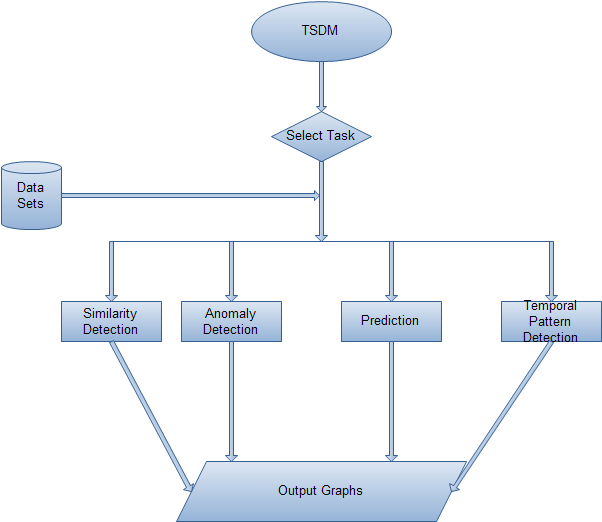
\includegraphics[scale=0.7]{system-architecture.png}
		\caption{ System Architecture}
\end{figure} 

\section{Data Flow Diagrams}
\paragraph{}A DFD is a figure which shows the flow of data between the different processes and how the data is modified in each of the process. It is very important tool in software engineering that is used for studying the high level design.\\
\paragraph{}There are many levels of DFDs. Level 0 gives the general description and level 1 gives the detailed description. Going higher in the level numbers greater description of the processes will be given.
\pagebreak
\subsection{DFD Level 0}
\paragraph{}The level 0 DFD is shown in Fig. 3.2 below which gives the general operation of the TSDM Tool. There are three major components. Two external entities called sender and receiver and the most important Time Series Data Mining Tool.
\begin{itemize}
\item Input Time Series Data : The user of this tool  is the one responsible to send the data to be analyzed using the tool. This tool can analyze only uni-variate time series data.
\item Analyzed Results: Depending the data sent by the user and the requested operations, the TSDM tool produces results in the form of graphs showing patterns, predictions, and other analyzed results.
\item TSDM Tool : This the software tool which is used to analyze the input time series data and generate meaningful results, patterns etc. depending on what the user wants.
\end{itemize}
\begin{figure}[h!]
	\centering
		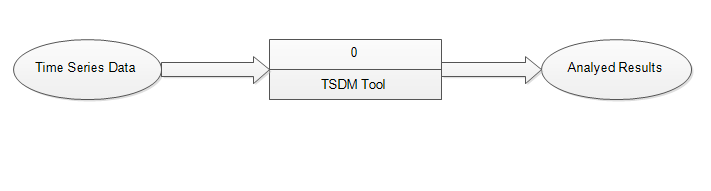
\includegraphics[scale=0.9]{screenshots/dfd_0.png}
		\caption{Data Flow Diagram Level 0}
\end{figure} 
\pagebreak
\subsection{DFD Level 1}
\paragraph{}Major components of the TSDM Tool are shown in  level 1 DFD as in Figure 3.3. The components are :

\noindent
The description of the modules are as below :
\begin{itemize}
\item \textbf{Similarity Detection} : This module helps in finding similarity patterns (that occur at regular intervals in case of periodic time series), comparing different time series data. SAX and DTW are the main algorithms implemented/used in this module.
\item \textbf{Forecasting and Prediction} : This module contain algorithms/models which can be trained from the past time series data and can be used to predict the future values of a time series. 
\item \textbf{Anomaly Detection} : This module contains algorithms that help in indicating anomalous patterns in the time series data analyzed. Anomalies are patterns in time series which deviate from the normal behavior and can indicate fraud/danger depending on the application. For example in an industry which produces the blades, the thickness of the blade can be monitored by a machine as a time series and any deviation from the normal error rate can signal an error in the manufacturing process.
\item \textbf{Temporal Pattern Finder } : This module helps in finding hidden temporal patterns in a time series. This module can be further extended to implement clustering techniques.
\end{itemize}

\noindent
Other components are 
\begin{itemize}
\item \textbf{Input } - Input is the uni-variate time series data to be analyzed using the tool.
\item \textbf{Output } - Output depends on the module selected by the user. This is visualized using the graphs/charts.
\end{itemize}
\begin{figure}[h!]
	\centering
		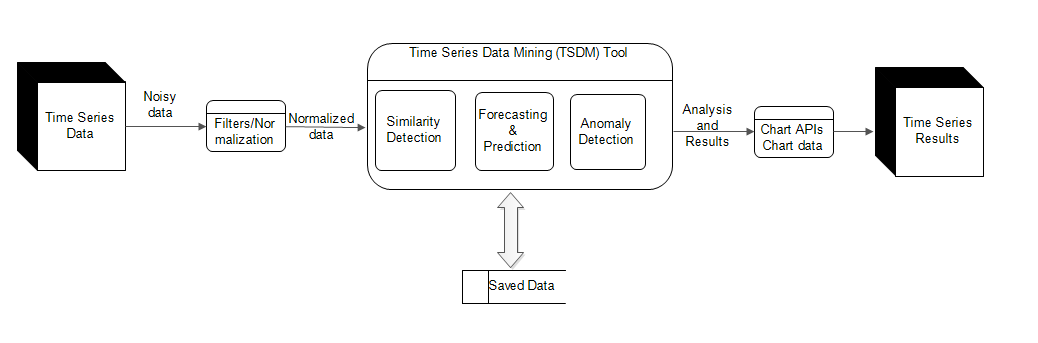
\includegraphics[scale=0.85]{screenshots/dfd_1.png}
		\caption{Data Flow Diagram Level 1}
\end{figure}

\subsubsection{DFD Level 1.1}
In DFD Level 1.1 shown in the figure 3.4, all the modules are expanded to show the algorithms implemented under them. The Input and the Output are same as level 1. Google charts are used for visualizing the results performed on the time series data.
\begin{figure}[h!]
	\centering
		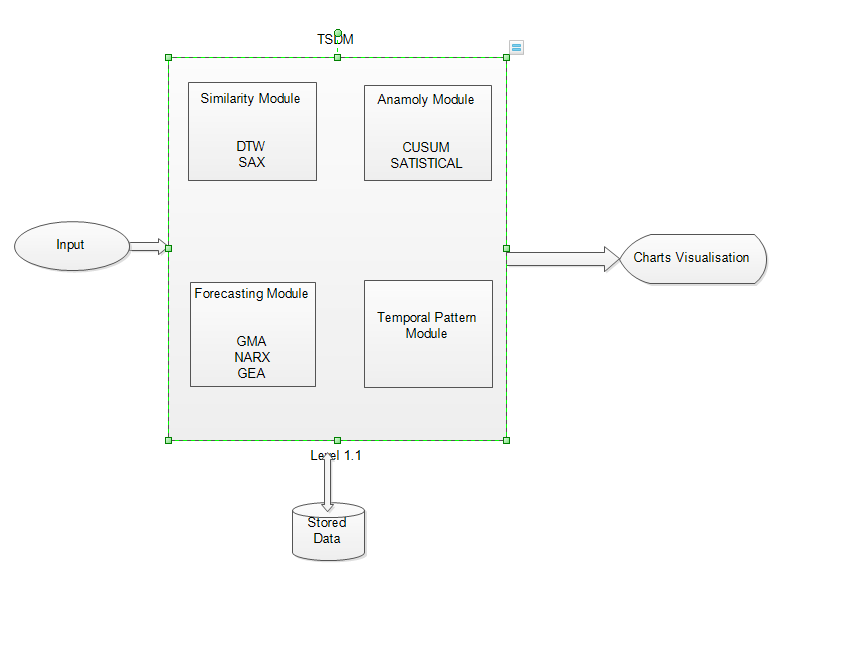
\includegraphics[scale=0.85]{screenshots/dfd_1_1.png}
		\caption{Data Flow Diagram Level 1.1}
\end{figure}
A brief description of the algorithms implemented under each module are below :
\begin{enumerate}

\item \textbf{Forecasting and Prediction}
\begin{itemize}
\item  NARX Neural Network : NARX is Non Linear Auto-Regressive with Extraneous Inputs. This is a neural network approach used for modeling a time series which depends on another time series. Back Propagation algorithm has been used to train the neural network.
Sigmoid activation function is  used for neurons. 
\end{itemize}

\item \textbf{Anomaly Detection }

\begin{itemize}
\item  Statistical Approach 
\item  CUSUM Approach 
\end{itemize}
These anomaly detection algorithms work in specific ways and help in determining the anomalous data points. The results are displayed in the output graphs.
\item \textbf{Similarity Detection }
\begin{itemize}
\item  DTW Algorithm : This algorithms helps in comparing two or more time series considering their euclidian distances and exhaustive comparing. This algorithm is computationally expensive but consumes less memory.
\item  SAX Algorithm : This algorithm converts the time series to a string and helps in comparing different time series and shows how similar the time series are by giving a similarity distance.
\end{itemize}

\item \textbf{Temporal Pattern Finder}
This module helps in determining interesting/temporal patterns in the time series data. The patterns are highlighted in the graphs.
\end{enumerate}

\subsection{DFD Level 2}
The DFD Level 2 diagram is shown in the Figure 3.5 . The Output that comes out of the TSDM tool is divided into various categories depending on the module and is as shown in the figure 3.5.
The output categories are :

\begin{figure}[h!]
	\centering
		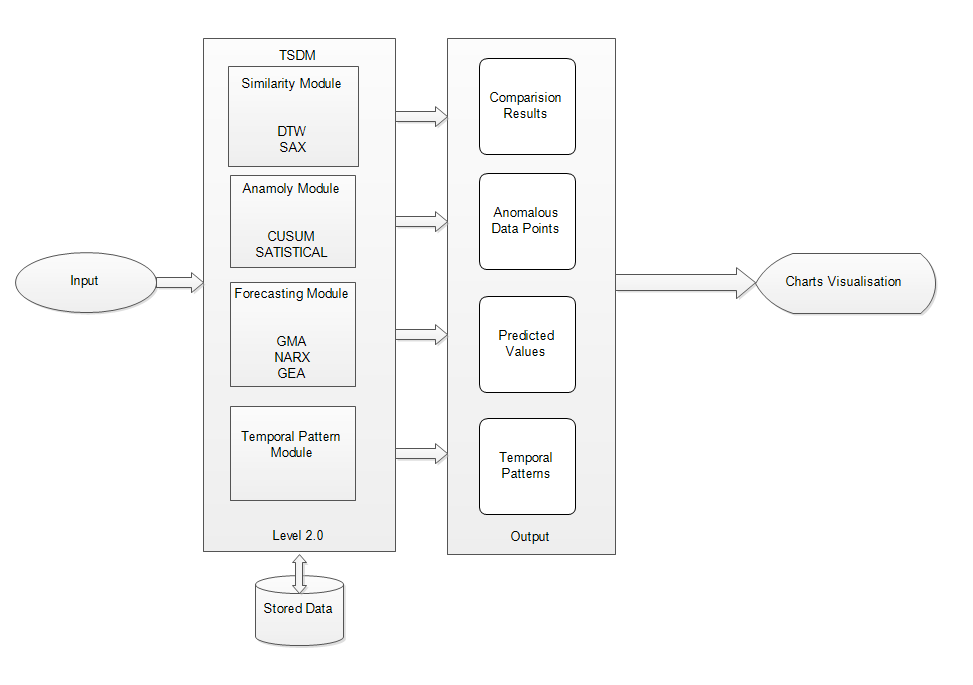
\includegraphics[scale=0.8]{screenshots/dfd_2.png}
		\caption{Data Flow Diagram Level 2}
\end{figure}
\begin{itemize}
\item Comparision Results  : The comparison results of the DTW or the SAX algorithm under the Similarity Detection Module are obtained and given as input to the charts api for visualization.
\item Anomalous Data Points  : The anomalous data points determined by the CUSUM or STATISTICAL algorithm under the Anomaly Detection Module are obtained and given as input to the charts application programmer interface for visualization.
\item Forecast/Predicted Results  : The predicted values of the input time series output by one of the NARX, GMA or GEA algorithms under the Forecasting Module are obtained and given as input to the charts api for visualization.
\item Temporal Patterns  : The temporal patterns found by the Temporal Pattern Finder module are obtained and given as input to the charts api for1 visualization.

\end{itemize}
\chapter{Detailed Design}
\pagestyle{fancy}
\lhead{\scriptsize{Detailed Design}}
\chead{}
\rhead{\scriptsize{Key Based Data Embedding Technique in Image Steganography}}
\lfoot{\scriptsize{Dept. of CSE, RVCE, Bangalore.}}
\rfoot{\small{\thepage}}
\cfoot{\scriptsize{September 2012 - January 2013}}
\renewcommand{\headrulewidth}{0.4pt}
\renewcommand{\footrulewidth}{0.4pt}
This chapter discusses the detailed design of the TSDM tool. In the section 4.1 the structured chart of the tool is explained.
\paragraph{}
In section 4.2 the details of the algorithms implemented under different modules of the tool are explained in detail.

\section{Structured Chart}
\paragraph{}Structure charts are used to specify the high level design or architecture of a computer program. As a design tool, they help the programmer in dividing and conquering a large software problem, i.e. recursively breaking a problem down into parts that are small enough to be understood by a human brain. The process is called top-down design or functional decomposition. 
\paragraph{}Programmers use a structure chart to build a program in a manner similar to how an architect uses a blueprint to build a house. In the design stage, the chart is drawn and used as a method for the client and various software designers to communicate. During the actual building of the program, the chart is continuously referred to as master plan. Often, it is modified as programmers learn new details about the program. After a program is completed, the structured chart is used to fix bugs and to make changes.


The structured chart for the TSDM tool is shown in the figure 4.1 The Output that comes out of the TSDM tool is divided into various categories depending on the module and is as shown in the figure 4.1.
The output categories are :

\begin{itemize}
\item Comparision Results  : The comparison results of the DTW or the SAX algorithm under the Similarity Detection Module are obtained and given as input to the charts API for visualization.
\item Anomalous Data Points  : The anomalous data points determined by the CUSUM or STATISTICAL algorithm under the Anomaly Detection Module are obtained and given as input to the charts API for visualization.
\item Forecast/Predicted Results  : The predicted values of the input time series output by one of the NARX, GMA or GEA algorithms under the Forecasting Module are obtained and given as input to the charts API for visualization.
\item Temporal Patterns  : The temporal patterns found by the Temporal Pattern Finder module are obtained and given as input to the charts API for visualization.
\end{itemize}
\begin{figure}[h!]
	\centering
		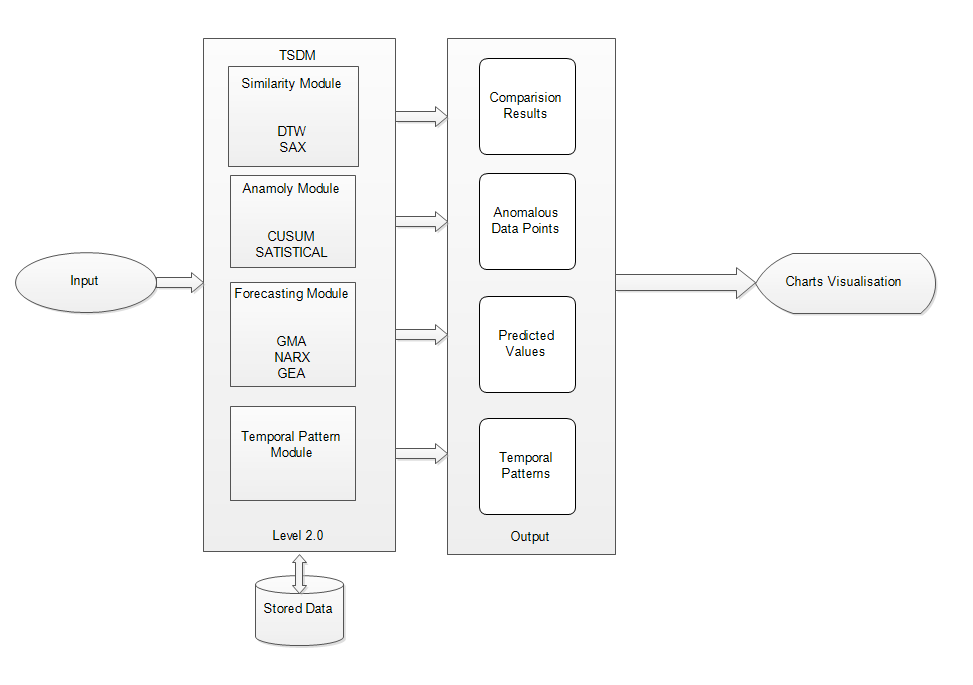
\includegraphics[scale=0.7]{screenshots/structured_chart.png}
		\caption{Structed Chart for the TSDM Tool }
\end{figure}

\section{Algorithm Details}
In this section, the algorithms implemented in the TSDM Tool are explained in required detail.

\paragraph{} As explained in the DFDs (figures 3.2 to 3.5), this tool mainly consists of four main modules.
The modules are as below :
\begin{itemize}
\item Similarity Detection Module
\item Forecasting and Prediction Module
\item Anomaly Detection Module
\item Temporal Pattern Finder 
\end{itemize}
\subsection{Similarity Detection Algorithms}
\subsubsection{Euclidian Distance}
One of the simplest similarity measures for time series is the Euclidean distance
measure. Assume that both time sequences are of the same length n, this sequence can be viewed as a point in n-dimensional Euclidean space, and define
the dissimilarity between sequences C and Q and D(C;Q) = $L_p(C;Q)$
i.e. the distance between the two points measured by the $L_p$ norm (when p = 2, it reduces to the familiar Euclidean distance). Figure 4.2 shows a visual intuition
behind the Euclidean distance metric.

\begin{figure}[h!]
	\centering
		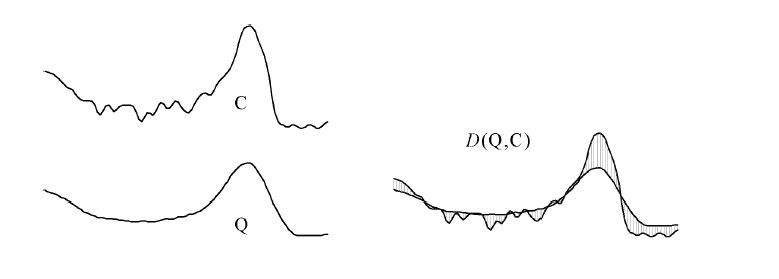
\includegraphics[scale=0.6]{screenshots/euclid.png}
		\caption{The intuition behind the Euclidean distance metric}
\end{figure}
Such a measure is simple to understand and easy to compute, which has ensured that the Euclidean distance is the most widely used distance measure for similarity search. However, one major disadvantage is that it is very brittle; it does not allow
for a situation where two sequences are alike, but one has been ``stretched" or ``compressed" in the Y -axis.

\subsubsection{DTW}
Dynamic time warping (DTW) is a well-known technique to find an optimal
alignment between two given (time-dependent) sequences under certain restrictions. Intuitively, the sequences are warped in a nonlinear fashion
to match each other. Originally, DTW has been used to compare different
speech patterns in automatic speech recognition. In fields such as
data mining and information retrieval, DTW has been successfully applied
to automatically cope with time deformations and different speeds associated
with time-dependent data.

\begin{figure}[h!]
	\centering
		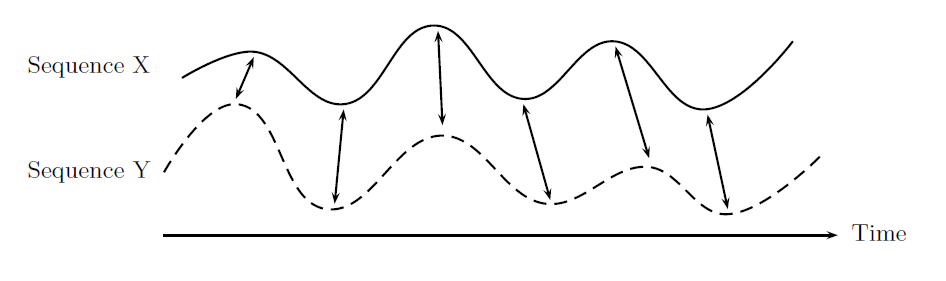
\includegraphics[scale=0.7]{screenshots/dtw/time_alignment.png}
		\caption{Time alignment of two time-dependent sequences.}
\end{figure}

The objective of DTW is to compare two (time-dependent) sequences 
$X := (x_1, x_2, . . . , x_N) $ of length $N \in N$ and $Y := (y_1, y_2, . . . , y_M)$ of length $M \in N$.\\
These sequences may be discrete signals (time-series) or, more generally, feature
sequences sampled at equidistant points in time. Fix a
feature space denoted by F. Then $x_n, y_m \in F$ for $n \in [1 : N]$ and  $m \in [1 : M].$\\
To compare two different features $x, y \in F$, one needs a local cost measure,
sometimes also referred to as local distance measure, which is defined to be a
function
c : $F \times F \rightarrow R. $
Typically, $c(x, y)$ is small (low cost) if x and y are similar to each other, and
otherwise $c(x, y$) is large (high cost).\\

\begin{figure}[h!]
	\centering
		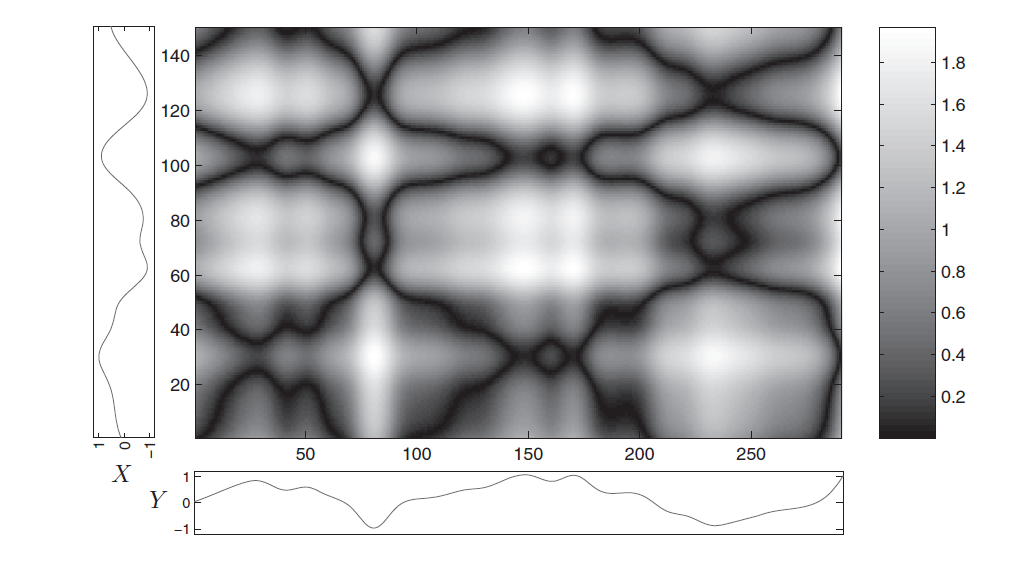
\includegraphics[scale=0.6]{screenshots/dtw/cost_matrix.png}
		\caption{Cost matrix of the two real-valued sequences X (vertical axis) and Y
(horizontal axis) using the Manhattan distance (absolute value of the difference) as
local cost measure c. Regions of low cost are indicated by dark colors and regions
of high cost are indicated by light colors}
\end{figure}

Evaluating the local cost measure for each pair of elements of the sequences X and Y , one obtains the cost matrix
$C \in R^{N \times M}$ defined by $C(n,m) := c(x_n, y_m)$. Then the goal is to
find an alignment between X and Y having minimal overall cost. Intuitively,
such an optimal alignment runs along a "valley" of low cost within the cost
matrix C.
\\

Basic Conditions to be satisfied:
An (N,M)-warping path (or simply referred to as warping
path if N and M are clear from the context) is a sequence $p = (p_1, . . . , p_L)$
with $p_l = (n_l,m_l) \in [1 : N] \times [1 : M] for l \in [1 : L]$ satisfying the following
three conditions.

\begin{enumerate}
\item{Boundary condition: $p_1 = (1, 1)$ and $p_L = (N,M).$}
\item{Monotonicity condition: $n_1 \leq n_2 \leq . . .  \leq n_L$ and $m_1 \leq m_2 \leq . . . \leq m_L.$}
\item{Step size condition:$ p_{l+1} − p_l \in {(1, 0), (0, 1), (1, 1)} $ for $l \in [1 : L − 1].$}
\end{enumerate}

\begin{figure}[h!]
	\centering
		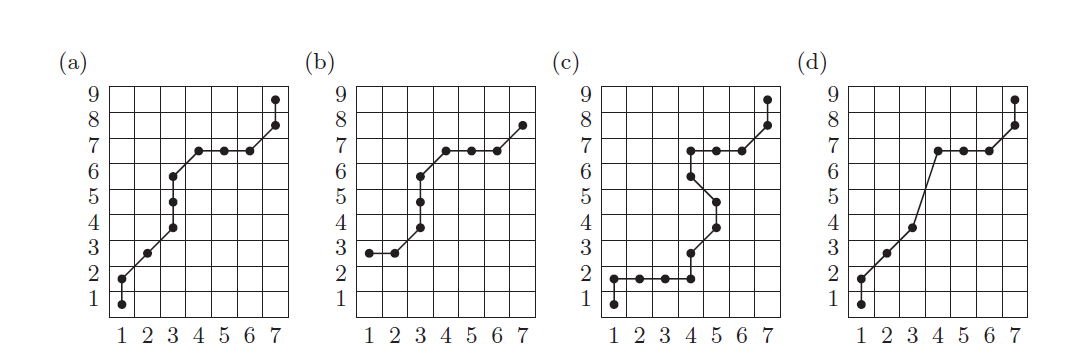
\includegraphics[scale=0.6]{screenshots/dtw/conditions.png}
		\caption{Illustration of paths of index pairs for some sequence X of length N = 9
and some sequence Y of length M = 7. (a) Admissible warping path satisfying the
conditions (i), (ii), and (iii) of Definition 4.1. (b) Boundary condition (i) is violated.
(c) Monotonicity condition (ii) is violated. (d) Step size condition (iii) is violated}
\end{figure}`
\subsubsection{SAX}
\subsection{Forecasting and Prediction Algorithms}
\subsubsection{NARX Neural Network}
\subsubsection{Moving Exponential Average Method}
Moving Exponential average,  is a technique that can be applied to time series data to produce smoothed data for presentation, or to make forecasts. Exponential smoothing is commonly applied to discrete set of repeated measurements. This makes it a method feasible for usage in the TSDM tool. Exponential smoothing was first suggested by Robert Goodell Brown in 1956, the one used in this tool is known as `` Brown's simple exponential smoothing".[14]
The algorithm is a trivial and the forecasting accuracy is not as good as the Neural network approach.
\subsubsection{Moving Geometric Average Method}
A moving average of order k, MA(k) is the value of k consecutive observations. A moving geometric  average is commonly used with time series data to smooth out short-term fluctuations and highlight longer-term trends or cycles. The method has  disadvantages. One of the important  disadvantage is that it is tough to extrapolate the values. This makes prediction inaccurate. [15]
\subsection{Anomaly Detection Algorithms}
\subsubsection{Cumulative Sum (CUSUM) Approach}
\subsubsection{Statistical Approach}
\subsection{Temporal Pattern Detection Algorithm}


\chapter{Implementation}
\pagestyle{fancy}
\lhead{\scriptsize{Implementation}}
\chead{}
\rhead{\scriptsize{Key Based Data Embedding Technique in Image Steganography}}
\lfoot{\scriptsize{Dept. of CSE, RVCE, Bangalore.}}
\rfoot{\small{\thepage}}
\cfoot{\scriptsize{September 2012 - January 2013}}
\renewcommand{\headrulewidth}{0.4pt}
\renewcommand{\footrulewidth}{0.4pt}
\paragraph{}The implementation phase of any project development is the most important phase and yields the final solution which solves the problem at hand.The implementation phase involves the actual materialization of the ideas, which are expressed in a suitable programming language. The factors concerning the programming language selection and platform chosen are described in the following sections.
\section{Programming Language Selection}

\paragraph{}The programming language chosen must reflect the necessities of the project to be completely expressed in terms of the analysis and the design documents. Therefore before choosing the language, features to be included in the project are decided. The time series data mining project needs the following features in a language to be implemented. Some of the features required are stated as follows:
\begin{itemize}
\item J2EE provides us with servlets and JSP which help in dynamically constructing web pages.
\item J2EE provides us with Java Beans which help in proper data manipulation.
\item JSP and servlets make use of Java backend in a very optimal manner. They have special tags which help us exploit these features.
\item Java's core classes are designed from scratch to meet the requirements of an object oriented system.
\end{itemize} 
With these necessities in mind, J2EE is selected as the optimal programming language to implement the project.
\section{Platform}
\paragraph{}The TSDM tool was built and designed on Windows Operating system family. They were specifically tested on Windows 7 with Google Chrome and Mozilla Firefox browsers. Because the product is browser based, any user with the browsers mentioned above will be able to run the tool. The product is hence platform independent in the true sense.
\section{Code Conventions}
\paragraph{}The code standards for the Java programming Language document contains the standard conventions that follows. It includes file names, file organizations, indentation, comments, declarations, naming conventions and programming practices. Code conventions improve the readability of the software.
\subsection{Naming Conventions}
 A naming convention is a set of rules for choosing the character sequence to be used for identifiers which denote variables, types, functions, and other entities in source code and documentation.  There are several common elements that influence most if not all naming conventions in common use today. They are :
\begin{itemize}
\item Use mixed case to make names readable
\item Avoid long names (15 characters maximum)
\item Avoid names that are too similar or that differ only in case
\item Capitalize the first letter of standard acronyms
\item Use terminology applicable to the domain
\item Use full descriptors that accurately describe the variable, field, or class
\end{itemize}
\subsection{File Organization}
As stated above, this project has been developed using the eclipse JEE IDE. This is a dynamic web project. The project has been organized as follows :
\begin{itemize}
\item\textbf{Java Resources} - This folder contains the java classes organized in packages. All the algorithms implemented in java are present in this folder under different packages.
\item\textbf{JavaScript Resources} - This folder contains the javascript library files.
\item\textbf{Web Content} - This folder mainly contains the jsp, js, html, css files which are used for developing the front webpages.
\end{itemize}

\subsection{Comments}
\begin{itemize}
\item{\textbf{Implementation Comment Formats}}
	\begin{itemize}
	\item \textbf{Block Comments}
	\begin{verbatim}
	/*
 	* Here is a block comment.
 	*/
	\end{verbatim}
	\item \textbf{Single Line Comments}
	\begin{verbatim}
	if (condition) {

    	/* Handle the condition. */
    	...
	}

	\end{verbatim}
	\item \textbf{Trailing Comments}
	\begin{verbatim}
	if (a == 2) {
 	   return TRUE;            /* special case */
	} else {
	    return isPrime(a);      /* works only for odd a */
	}
	\end{verbatim}
	\item \textbf{End-of-Line Comments}
	\begin{verbatim}
	if (foo > 1) {

    // Do a double-flip. Harlem Style
    	...
	}
	else	 {
    	return false;          // Explain why here.	
	}
	\end{verbatim}
	\end{itemize}
\item{\textbf{Documentation Comments}}
\begin{verbatim}
/**
 * The Example class provides ...
 */
public class Example { ...
\end{verbatim}

\end{itemize}
\section{Difficulties encountered and Strategies used to tackle}

\paragraph{}There were a number of challenges that were faced while implementing the Time Series Data Mining tool.Some challenges were challenging and ended up in helping us think innovatively and come up with efficient solutions. Some major problems that were encountered have been stated in brief along with their solutions.
\subsubsection{Problem 1}
\paragraph{}Initially the front end was designed in python using django web framework. But integrating java (back-end) with python had performance issues.(Using Jython interpreter)
\subsubsection{Solution}
\paragraph{}JSP (Java server pages) was later used for the front end and this problem was solved.
\subsubsection{Problem 2}
\paragraph{}In the initial stages of the project charts4j libraries were used to plot graphs. There were some internal problems with the URL rendering.

\subsubsection{Solution}
\paragraph{}This Problem was solved later by making use of Google's Charts API and java script. 


\section{Module Design}

Object-oriented programming (OOP) is a programming paradigm that represents concepts as ``objects" that have data fields (attributes that describe the object) and associated
procedures known as methods. Objects, which are instances of classes, are used to interact with one another to design applications and computer programs.
In this chapter, we describe the different packages that were created by us to efficiently manage our code. Know first that our application consists of four diverse packages, namely:\textbf{}
\textit{\begin{enumerate}
\itemsep-0.5em
\item{org.ck.sample}
\item{org.ck.smoother}
\item{org.ck.similarity}
\item{org.ck.forecaster.nn}
\item{org.ck.anomalifinder}
\item{org.ck.tsdm}
\item{org.ck.tsdm.ga}
\item{org.ck.beans}
\item{org.ck.servlets}
\item{org.ck.gui}
\end{enumerate}}

Each package is explained  in detail, in the following sections. A bottom-up methodology is followed for explaining the layout of the classes.

\subsection{org.ck.sample}
This package allows us to efficiently manage and encapsulate the details of the data
samples, provided by users, which are required for analysis. It is this class that allows our application to accept generic data sets. It consists of four classes:

\begin{enumerate}
\item{\textbf{DataHolder} - This class keeps track of names of files that contain time series data; the fitness score threshold for the genetic algorithm. It provides this information, when required, to the front-end or back-
end of our application. To make a long story short, this class acts like a middleman
between the back-end and front-end of our application.}

\item{\textbf{Sample} - This class stores the values of a given time series in various forms - discrete and continuous; normalized and unnormalized; smooth and unsmooth; SAX Representation. It keeps track of all dimensions of a given time-series }



\end{enumerate}

\subsection{org.ck.smoothers}
This package consists of a number of smoothing filters that can be used to smoothen time series values stored in an object of the Sample class. These classes also double up as naive forecaster modules. They are based on the concept of Moving Averages.

\begin{enumerate}
\item{\textbf{SmoothingFilter} - This is the parent class of all the other classes in this package. It is also an abstract class. Hence, all the other classes that extend this class must provide implementations for the calculateSmoothedValues() and getAverage() methods compulsorily.}

\item{\textbf{ExponentialMovingAverageSmoother} - This class extends the SmoothingFilter class. Exponential smoothing is commonly applied to financial market and economic data, but it can be used with any discrete set of repeated measurements. The raw data sequence is often represented by $x_t$, and the output of the exponential smoothing algorithm is commonly written as $s_t$, which may be regarded as a best estimate of what the next value of x will be. When the sequence of observations begins at time t = 0, the simplest form of exponential smoothing is given by the formulae:

$s_0 = x_0$
$s_t = \alpha x_t + (1 - \alpha) * s_{t-1} , t > 0$

where $\alpha$ is the smoothing factor, and $0 < \alpha < 1$.}

\item{\textbf{SimpleMovingAverageSmoother} - This class extends the SmoothingFilter class. A simple moving average (SMA) is the unweighted mean of the previous n datum points.

$SMA = (t_m + t_{m-1} + t_{m-2} + t_{m-3} + ... + t_{m-(n-1)}) \div n$

where $t_m$ is the value of the time series at the $m^{th}$ instance of time.

}

\item{\textbf{GeometricMovingAverageSmoother} - This class extends the SmoothingFilter class.The Geometric moving average calculates the geometric mean of the previous N bars of a time series.}

\end{enumerate}

\subsection{org.ck.similarity}
This module helps in finding similarity patterns (that occur at regular intervals in case of periodic time series), comparing different time series data. SAX and DTW are the main algorithms implemented/used in this module.

\begin{enumerate}
\item{\textbf{DynamicTimeWarper} - Dynamic time warping (DTW) is an algorithm for measuring similarity between two sequences which may vary in time or speed. In general, DTW is a method that allows a computer to find an optimal match between two given sequences (e.g. time series) with certain restrictions. The sequences are "warped" non-linearly in the time dimension to determine a measure of their similarity independent of certain non-linear variations in the time dimension. This sequence alignment method is often used in time series classification. This class implements the aforementioned functionality.}

\item{\textbf{Discretizer} - This Singleton class is used to convert a time series represented by a PAA (Piecewise Aggregate Approximation), to a string representation (SAX - Symbolic Aggregate Approximation)}

\item{\textbf{Approximator} - This class averages out any time series containing continuous values using Piecewise Aggregate Approximation, allowing the time series to occupy as small a space as possible.}

\end{enumerate}


\subsection{org.ck.forecaster.nn}

This package contain algorithms/models which can be trained from the past time series data and can be used to predict the future values of a time series. In more practical terms neural networks are non-linear statistical data modeling or decision making tools. They can be used to model complex relationships between inputs and outputs or to find patterns in data.



\begin{enumerate}

\item{\textbf{Neuron}} - In a neural network model simple nodes (which can be called by a number of names, including ``neurons", ``neurodes", ``Processing Elements" (PE) and ``units"), are connected together to form a network of nodes — hence the term ``neural network".
\item{\textbf{NetworkLayer}} - Creating the neural network architecture therefore means coming up with values for the number of layers of each type and the number of nodes in each of these layers.

\begin{itemize}
\item{The Input Layer}
\item{The Hidden Layer}
\item{The Output Layer}
\end{itemize}


\item{\textbf{NeuralNetwork}} - A neural network (NN), in the case of artificial neurons called artificial neural network (ANN) or simulated neural network (SNN), is an interconnected group of natural or artificial neurons that uses a mathematical or computational model for information processing based on a connectionistic approach to computation.


\end{enumerate}

\subsection{org.ck.anomalifinder}
\paragraph{} This package contains algorithms that help in indicating anomalous patterns in the time series data analyzed. Anomalies are patterns in time series which deviate from the normal behavior and can indicate fraud/danger depending on the application. For example in an industry which produces the blades, the thickness of the blade can be monitored by a machine as a time series and any deviation from the normal error rate can signal an error in the manufacturing process.

\begin{enumerate}

\item{\textbf{Cusum\_VmaskApproch}}

\item{\textbf{CusumAnomalyMethod}}

\end{enumerate}

\subsection{org.ck.tsdm}

\paragraph{} This package contains a set of classes that reveal hidden
patterns in time series data and overcome limitations of traditional time series analysis
techniques. This Temporal Pattern Mining tool focuses on predicting events, which are important
occurrences. This allows the TSDM methods to predict nonstationary, nonperiodic,
irregular time series, including chaotic deterministic time series. It makes use of a genetic algorithm, internally.

\begin{enumerate}

\item{\textbf{TSDM} - This class is to be used to find Temporal Patterns in Time Series and maintains status information about the algorithm.}

\item{\textbf{PhaseSpace} - Represents a Q-Dimensional Phase Space of points in the time series}

\item{\textbf{PhasePoint} - A point in a Q-Dimensional Phase Space}

\end{enumerate}

\subsection{org.ck.tsdm.ga}
This package takes care of all operations of the Genetic algorithm that is used by the TSDM class of the org.ck.tsdm package.

\begin{enumerate}
\item{\textbf{Genome} - This class takes as input, a chromosome that encodes a given phase space cluster. It keeps track of this chromosome, and provides methods to manipulate
this chromosome; to calculate the fitness score of this chromosome; and to throw an
exception when the fitness value threshold has been crossed or when the best solution has been discovered.}


\item{\textbf{Population} - As defined earlier, a population is a collection of genomes. And this is
exactly what this class is. Initially, the Population class randomly initializes a large
number of genomes, of which it keeps track. It provides methods such as roulette
selection, reproduction, crossover, and mutation to operate on the population and
discover the best genome, and hence, the best decision tree with the appropriate
feature subset.}


\item{\textbf{OptimalScoreException} - This class is responsible for catching the best genome
as soon as it is discovered, since the best genome should never be allowed to escape.
It should be caught and nurtured for future use.}

\end{enumerate}

\subsection{org.ck.beans}

JavaBeans are reusable software components for Java. Practically, they are classes that encapsulate many objects into a single object (the bean). They are serializable, have a 0-argument constructor, and allow access to properties using getter and setter methods.

\begin{enumerate}

\item{\textbf{TimeSeriesBean} - This bean stores information about requested values and results of calculations. The results produced by the Similarity, Forecaster, Anomaly Detection and Temporal Pattern Mining modules are stored in an object of this class, and the front-end reads the results from this bean. It is our very own custom class that allows any number of user-defined objects to be stored for communication.}

\end{enumerate}

\subsection{org.ck.servlets}

A Servlet is an object that receives a request and generates a response based on that request. 

\begin{enumerate}

\item{\textbf{MainController} - This servlet is the controller that gets requests from JSP pages, generates results through beans and forwards them to other jsp pages.}

\item{\textbf{AlgorithmUtils} - This class is a utility class that contains methods to run various algorithms in this tool.}

\end{enumerate}

\subsection{org.ck.gui}

This package allows each member of our team to test out the functionality of the back-end framework before connecting to the front-end to it.

\begin{enumerate}

\item{\textbf{Constants} - A number of constants and enumerations used by all the other classes and packages.}

\item{\textbf{MainClass} - After a method is added to any class, the method is called from the respective team member's method to test it. If it works fine, then the tested method is used in the front-end.}

\end{enumerate}

\pagestyle{fancy}
\lhead{\scriptsize{Software Testing}}
\chead{}
\rhead{\scriptsize{Time Series Data Mining Tool}}
\lfoot{\scriptsize{Dept. of CSE, RVCE, Bangalore.}}
\rfoot{\small{\thepage}}
\cfoot{\scriptsize{Jan 2013 - Jun 2013}}
\renewcommand{\headrulewidth}{0.4pt}
\renewcommand{\footrulewidth}{0.4pt}
\chapter{Software Testing}

The purpose of testing is to discover errors. Testing is the process of trying to
discover every conceivable fault or weakness in a work product. It provides a way to
check the functionality of components, sub assemblies, assemblies and/or a finished
product Testing is the process of exercising software with the intent of ensuring that
the Software system meets its requirements and user expectations and does not fail in
an unacceptable manner. There are various types of test. Each test type addresses a
specific testing requirement.
\section{Types Of Testing}
\subsubsection{Unit testing}
Unit testing involves the design of test cases that validate that the internal
program logic is functioning properly, and that program input produces valid outputs.
All decision branches and internal code flow should be validated. It is the testing of
individual software units of the application. It is done after the completion of an
individual unit before integration. This is a structural testing, that relies on knowledge
of its construction and is invasive. Unit tests perform basic tests at component level
and test a specific business process, application, and/or system configuration. Unit
tests ensure that each unique path of a business process performs accurately to the
documented specifications and contains clearly defined inputs and expected results.
\subsubsection{Integration testing}
Integration tests are designed to test integrated software components to
determine if they actually run as one program. Testing is event driven and is more
concerned with the basic outcome of screens or fields. Integration tests demonstrate
that although the components were individually satisfaction, as shown by successfully
unit testing, the combination of components is correct and consistent. Integration
testing is specifically aimed at exposing the problems that arise from the combination
of components.
\subsubsection{Functional test}
Functional tests provides a systematic demonstration that functions tested are
available as specified by the business and technical requirements, system
documentation, and user manuals. Functional testing is centered on the following
items:
Valid Input: identified classes of valid input must be accepted.
Invalid Input: identified classes of invalid input must be rejected.
Functions: identified functions must be exercised.
Output: identified classes of application outputs must be exercised.
Systems / Procedures: interfacing systems or procedures must be invoked.
Organization and preparation of functional tests is focused on requirements,
key functions, or special test cases. In addition, systematic coverage pertaining to
identifying business process flows, data fields, predefined processes, and successive
processes must be considered for testing. Before functional testing is complete,
additional tests are identified and the effective value of current tests is determined.
\subsubsection{System Test}
System testing ensures that the entire integrated software system meets
requirements. It tests a configuration to ensure known and predictable results. An
example of system testing is the configuration oriented system integration test.
System testing is based on process descriptions and flows, emphasizing pre-driven
process links and integration points.
\subsubsection{Performance Test}
The Performance test ensures that the output be produced within the time
limits, and the time taken by the system for compiling, giving response to the users
and request being send to the system for to retrieve the results.
\subsubsection{White Box Testing}
White Box Testing is a testing in which in which the software tester has
knowledge of the inner workings, structure and language of the software, or at least its
purpose. It is used to test areas that cannot be reached from a black box level.
\subsubsection{Black Box Testing}
Black Box Testing is testing the software without any knowledge of the inner
workings, structure or language of the module being tested. Black box tests, as most
other kinds of tests, must be written from a definitive source document, such as
specification or requirements document, such as specification or requirements
document. It is a testing in which the software under test is treated, as a black box
.you cannot “see” into it. The test provides inputs and responds to outputs without
considering how the software works.
%\section{Test Environment}
\section{Test Environment}
The testing of the modules was done on machine with the following features.
\begin{description}
  \item[Operating System ] : Windows 7 
  \item[JDK Version ] : 1.7 
  \item[Browser ] : Google Chrome 
  \item[Web server ]: Tomcat Version 7 
\end{description}
\newpage


\begin{table}
    \begin{tabular}{|l|l|}
    \hline
    Sl. Number of Test Case & 1                                  \\ \hline
    Name Of the test        & Connection between Tomcat and JDK. \\ \hline
    Feature Being Tested    & Tomcat Instance Working            \\ \hline
    Input                   & Tomcat Catalina Home batch file    \\ \hline
    Expected Output         & Home Page Must Open                \\ \hline
    Output                  & Home Page Opens                    \\ \hline
    Remarks                 & Test case passed                   \\ \hline
    \end{tabular}
    \caption {Test Case 1 - System Test}
\end{table}



%\subsubsection{Test Case 2}
\begin{table}
    \begin{tabular}{|l|l|}
    \hline
    Sl. Number of Test Case & 2                                                      \\ \hline
    Name Of the test        & Working of JQuery and Ajax Libraries                   \\ \hline
    Feature Being Tested    & Presence of JQuery Libraries and Ajax Libraries        \\ \hline
    Input                   & Nil                                                    \\ \hline
    Expected Output         & Home Page Must Open with Jquery and Ajax Functionality \\ \hline
    Output                  & Home Page Opens as expected                            \\ \hline
    Remarks                 & Test case passed                                       \\ \hline
    \end{tabular}
    \caption {Test Case 2 - System Test}
\end{table}





\begin{table}
    \begin{tabular}{|l|l|}
    \hline
    Sl. Number of Test Case & 3                                  \\ \hline
    Name Of the test        & Working of Google Charts API       \\ \hline
    Feature Being Tested    & Charts                             \\ \hline
    Input                   & Data Files                         \\ \hline
    Expected Output         & Scatter and Line Plots must appear \\ \hline
    Output                  & Charts are plotted                 \\ \hline
    Remarks                 & Test case passed                   \\ \hline
    \end{tabular}
    \caption {Test Case 3 - System Test}
\end{table}



\begin{table}
    \begin{tabular}{|l|l|}
    \hline
    Sl. Number of Test Case & 4                             \\ \hline
    Name Of the test        & Network Testing               \\ \hline
    Feature Being Tested    & Checking Network Connectivity \\ \hline
    Input                   & IP address of any DNS server  \\ \hline
    Expected Output         & Ping Data                     \\ \hline
    Output                  & Ping Data Obtained            \\ \hline
    Remarks                 & Test case passed              \\ \hline
    \end{tabular}
    \caption {Test Case 4 - Integration Test}
\end{table}

\begin{table}
    \begin{tabular}{|l|l|}
    \hline
    Sl. Number of Test Case & 5                             \\ \hline
    Name Of the test        & Performance Testing               \\ \hline
    Feature Being Tested    & Performance of various algorithms in the tool\\ \hline
    Input                   & Time series data specified by the user  \\ \hline
    Expected Output         & Load the graphs/results within the timeout specified.   \\ \hline
    Output                  & visualization graphs appear           \\ \hline
    Remarks                 & Test case passed              \\ \hline
    \end{tabular}
    \caption {Test Case 5 - Performance Test}
\end{table}

\begin{table}
    \begin{tabular}{|l|l|}
    \hline
    Sl. Number of Test Case & 6                             \\ \hline
    Name Of the test        & Load Testing               \\ \hline
    Feature Being Tested    & Memory consumption of the tool per request\\ \hline
    Input                   & Time series data and operations specified by the user  \\ \hline
    Expected Output         & Process maximum requests from the users \\ \hline
    Output                  & server computer handle multiple requests \\ \hline
    Remarks                 & Test case passed              \\ \hline
    \end{tabular}
    \caption {Test Case 6 - Load Test}
\end{table}

\begin{table}
    \begin{tabular}{|l|l|}
    \hline
    Sl. Number of Test Case & 7                             \\ \hline
    Name Of the test        & DTW Algorithm Testing        \\ \hline
    Feature Being Tested    & Working of the DTW Algorithm \\ \hline
    Input                   & A null value time series is passed as a parameter\\ \hline
    Expected Output         & Similarity distance of -1 \\ \hline
    Output                  & A Java.NullPointer Exception is thrown \\ \hline
    Remarks                 & Test case failed              \\ \hline
    \end{tabular}
    \caption {Test Case 7 - Similarity DTW Algorithm.}
\end{table}
\begin{table}
    \begin{tabular}{|l|l|}
    \hline
    Sl. Number of Test Case & 8                            \\ \hline
    Name Of the test        & DTW Algorithm Testing        \\ \hline
    Feature Being Tested    & Working of the DTW Algorithm \\ \hline
    Input                   & same Time series data for both parameters\\ \hline
    Expected Output         & Similarity distance of 0 \\ \hline
    Output                  & Similarity distance of 0 \\ \hline
    Remarks                 & Test case passed              \\ \hline
    \end{tabular}
    \caption {Test Case 8 - Similarity DTW Algorithm.}
\end{table}


\begin{table}
    \begin{tabular}{|l|l|}
    \hline
    Sl. Number of Test Case & 9                            \\ \hline
    Name Of the test        & SAX Algorithm Testing        \\ \hline
    Feature Being Tested    & Working of the DTW Algorithm \\ \hline
    Input                   & same Time series data for both parameters\\ \hline
    Expected Output         & Similarity distance of 0 \\ \hline
    Output                  & Similarity distance of 0 \\ \hline
    Remarks                 & Test case passed              \\ \hline
    \end{tabular}
    \caption {Test Case 9 - Similarity SAX Algorithm.}
\end{table}

\begin{table}
    \begin{tabular}{|l|l|}
    \hline
    Sl. Number of Test Case & 10                            \\ \hline
    Name Of the test        & Testing Temporal Pattern Detection Algorithm \\ \hline
    Feature Being Tested    & Temporal Pattern Detection Module \\ \hline
    Input                   & Time series data with threshold value 5.0\\ \hline
    Expected Output         & Temporal patterns \\ \hline
    Output                  & Improper patterns are shown \\ \hline
    Remarks                 & Test case failed             \\ \hline
    \end{tabular}
    \caption {Test Case 10 : Testing Temporal Pattern Detection}
\end{table}
\begin{table}
    \begin{tabular}{|l|l|}
    \hline
    Sl. Number of Test Case & 11                            \\ \hline
    Name Of the test        & Testing Anomaly Detection Algorithm\\ \hline
    Feature Being Tested    & Statistical Approach  \\ \hline
    Input                   & Time series data with a low threshold value\\ \hline
    Expected Output         & Large number of anomalous data points \\ \hline
    Output                  & Large number of anomalous points shown \\ \hline
    Remarks                 & Test case passed             \\ \hline
    \end{tabular}
    \caption {Test Case 11 - Testing Anomaly Detection}
\end{table}
\begin{table}
    \begin{tabular}{|l|l|}
    \hline
    Sl. Number of Test Case & 12                            \\ \hline
    Name Of the test        & Testing Anomaly Detection Algorithm\\ \hline
    Feature Being Tested    & Statistical Approach  \\ \hline
    Input                   & Time series data with a higher threshold value\\ \hline
    Expected Output         & Number of anomalous data points decrease \\ \hline
    Output                  & Number of anomalous points reduce \\ \hline
    Remarks                 & Test case passed             \\ \hline
    \end{tabular}
    \caption {Test Case 12 - Testing Anomaly Detection}
\end{table}
\begin{table}
    \begin{tabular}{|l|l|}
    \hline
    Sl. Number of Test Case & 13                           \\ \hline
    Name Of the test        & SAX Algorithm Testing        \\ \hline
    Feature Being Tested    & Working of the DTW Algorithm \\ \hline
    Input                   & same Time series data for both parameters\\ \hline
    Expected Output         & Similarity distance of 0 \\ \hline
    Output                  & Similarity distance of 0 \\ \hline
    Remarks                 & Test case passed              \\ \hline
    \end{tabular}
    \caption {Test Case 13 - Testing Anomaly Detection.}
\end{table}

\begin{table}
    \begin{tabular}{|l|l|}
    \hline
    Sl. Number of Test Case & 14                            \\ \hline
    Name Of the test        & Testing Forecasting Module     \\ \hline
    Feature Being Tested    & Working of the Moving Exponential Algorithm \\ \hline
    Input                   & Time series and expected predictions as parameters\\ \hline
    Expected Output         & The predictions match as per the parameter sent \\ \hline
    Output                  & predictions match \\ \hline
    Remarks                 & Test case passed              \\ \hline
    \end{tabular}
    \caption {Test Case 14 - Forecasting Moving Exponential Average.}
\end{table}
\begin{table}
    \begin{tabular}{|l|l|}
    \hline
    Sl. Number of Test Case & 15                            \\ \hline
    Name Of the test        & Testing Forecasting Module     \\ \hline
    Feature Being Tested    & Working of the Moving Exponential Algorithm \\ \hline
    Input                   & An empty/null time series is passed\\ \hline
    Expected Output         & null value to be returned for predictions \\ \hline
    Output                  & NullPointer Exception is thrown \\ \hline
    Remarks                 & Test case failed              \\ \hline
    \end{tabular}
    \caption {Test Case 15 - Forecasting Moving Exponential Average.}
\end{table}
\begin{table}
    \begin{tabular}{|l|l|}
    \hline
    Sl. Number of Test Case & 16                            \\ \hline
    Name Of the test        & Testing Forecasting Module     \\ \hline
    Feature Being Tested    & Working of the Moving Geometric Algorithm \\ \hline
    Input                   & Time series and expected predictions as parameters\\ \hline
    Expected Output         & The predictions match as per the parameter sent \\ \hline
    Output                  & predictions match \\ \hline
    Remarks                 & Test case passed              \\ \hline
    \end{tabular}
    \caption {Test Case 16 - Forecasting Moving Geometric Average.}
\end{table}
\begin{table}
    \begin{tabular}{|l|l|}
    \hline
    Sl. Number of Test Case & 17                            \\ \hline
    Name Of the test        & Testing Forecasting Module     \\ \hline
    Feature Being Tested    & Working of the Moving Geometric Algorithm \\ \hline
    Input                   & An empty/null time series is passed\\ \hline
    Expected Output         & null value to be returned for predictions \\ \hline
    Output                  & null value is returned \\ \hline
    Remarks                 & Test case passed.             \\ \hline
    \end{tabular}
    \caption {Test Case 17 : Forecasting Moving Geometric Average.}
\end{table}

\begin{table}
    \begin{tabular}{|l|l|}
    \hline
    Sl. Number of Test Case & 18                            \\ \hline
    Name Of the test        & Testing Forecasting Module     \\ \hline
    Feature Being Tested    & Working of the NARX Neural Network \\ \hline
    Input                   & Time series data with learning rate 1.0\\ \hline
    Expected Output         & Prediction accuracy of 70\% \\ \hline
    Output                  & Prediction accuracy is 20\% \\ \hline
    Remarks                 & Test case failed.             \\ \hline
    \end{tabular}
    \caption {Test Case 18 - Forecasting with NARX Neural Network.}
\end{table}

\pagestyle{fancy}
\lhead{\scriptsize{Experimental Analysis and Results}}
\chead{}
\rhead{\scriptsize{Time Series Data Mining Tool}}
\lfoot{\scriptsize{Dept. of CSE, RVCE, Bangalore.}}
\rfoot{\small{\thepage}}
\cfoot{\scriptsize{Jan 2013 - Jun 2013}}
\renewcommand{\headrulewidth}{0.4pt}
\renewcommand{\footrulewidth}{0.4pt}
\chapter{Experimental Analysis and Results}
In this chapter, all the performance and experimental analysis of the algorithms implemented under various different modules and the results obtained are presented.
\section{Evaluation Metric}
As explained earlier, major module present in the project are as follows :
\begin{itemize}
\item Similarity Detection Module
\item Prediction and Forecasting Module
\item Anomaly Detection Module
\item Temporal Pattern Finder Module
\end{itemize}

Since these modules are independent of each other, they have different evaluation metrics. The evaluation metrics used for performance analysis of each module is explained in the following sub sections.

\subsection{Metrics for Similarity Detection Module}
The algorithms implemented under this module are :
\begin{itemize}
\item \textbf{Dynamic Time Wrapping (DTW) Algorithm}
\item \textbf{SAX Algorithms}
\end{itemize}
The evaluation metrics are :
\begin{itemize}
\item \textbf{Euclidean Distance} In mathematics, the Euclidean distance or Euclidean metric is the ``ordinary" distance between two points that one would measure with a ruler, and is given by the Pythagorean formula. By using this formula as distance, Euclidean space (or even any inner product space) becomes a metric space. The associated norm is called the Euclidean norm. Older literature refers to the metric as Pythagorean metric.



In Cartesian coordinates, if p = $(p_1, p_2,..., p_n)$ and q = $(q_1, q_2,..., q_n)$ are two points in Euclidean n-space, then the distance from p to q, or from q to p is given by:
$$d(p,q)=d(q,p)=\sqrt{(p_1-q_1)^2+(p_2-q_2)^2+....+(p_n-q_n)^2} $$
$$d(p,q)=d(q,p)=\sqrt{\sum_{i=0}^{n}{(p_i-q_i)^2}}$$


In the project, p and q can be visualized as two time series to be compared, where $p_i$\'s and $q_i$\'s are the time series values.
Depending on the distance, the similarity of two or more time series with a give base series is found out. This metric is used in the DTW approach.
\item \textbf{String Comparison} In SAX Algorithm, the time series is converted into a string of character as explained. Given two or more time series, which are represented by strings, a string comparison algorithm is run and the similarity is found out. There are various string comparison algorithms. In this project KMP algorithm has been used.
\end{itemize}
\subsection{Metrics for Prediction and Forecasting Module}
The algorithms implemented under this module for modeling and forecasting time series are :
\begin{itemize}
\item NARX-Neural Network
\item Moving Average Forecaster
\item Moving Geometric Average Forecaster
\item Moving Exponential Average Forecaster
\end{itemize}
Modeling a time series is an regression problem, the evaluation metrics are :
\begin{itemize}
\item \textbf{Root-Mean-Square Deviation} - The root-mean-square deviation (RMSD) or root-mean-square error (RMSE) is a frequently used measure of the differences between values predicted by a model or an estimator and the values actually observed. These individual differences are called residuals when the calculations are performed over the data sample that was used for estimation, and are called prediction errors when computed out-of-sample. The RMSD serves to aggregate the magnitudes of the errors in predictions for various times into a single measure of predictive power. RMSD is a good measure of accuracy, but only to compare forecasting errors of different models for a particular variable and not between variables, as it is scale-dependent.




The RMSD of predicted values $y_p$ for times t of a regression's dependent variable $y$ is computed for n different predictions as the square root of the mean of the squares of the deviations:
$$RMSD=\sqrt{\sum_{i=0}^{n}{(y_p-y)^2/n}}$$

The accuracies  of different algorithms are compared and presented in the next section.
\end{itemize}
\subsection{Metrics for Anomaly Detection  Module}
The anomaly detection algorithms require the controller/user to specify various parameters which determine the anomalous points in the time series.


Algorithms implemented under this module are :
\begin{itemize}
\item \textbf{Cumulative Sum Approach (CUSUM)}
\item \textbf{Statistical Approach}
\end{itemize}

These algorithms require a \textbf{threshold value} to be specified by the user and depending on this value, anomalous data points are determined.
\subsection{Temporal Pattern Finder Module}
\paragraph{} In this module, a Genetic Algorithm has been implemented to optimize the algorithm. The fitness function used in the GA determine the accuracies of the patterns found. But eventually user intervention is required to interpret the resulting patterns detected by the algorithm. The results are documented in the next section.
\section{Experimental Dataset}
The data sets considered in this project are
\begin{itemize}
\item Sea Level Dataset : Indicating the sea level at various times of a day.
\item Water Level : Ground Water level data, indicating the ground water level during various moths of an year for upto 5 years.
\item Finance Dataset : Consisting of stock index values of  Nifty and Vix collected every minuted for a week.(5 days,during market hours).
\item ECG Dataset : The ECG  voltage values of patients collected every 4ms.(for 10 patients).
\end{itemize}
All the experiment analysis and results are presented using the \textbf{Water Level} data set. As explained earlier, some algorithms require certain parameters which determine their accuracies.
\section{Performance Analysis}
\paragraph{} In the previous section, the evaluations metrics for different modules depending on the algorithm were explained. Performance analysis of different modules implemented in this project are explained in the following sub sections
\subsection{Similarity Detection}
\subsubsection{DTW Algorithm }
\paragraph{} The working of the DTW algorithm for comparing two samples of same size in different intervals is shown in the figure 7.1. The data sets compared are the rainfall levels in the period 2001 to 2010. The former five years data is compared with the latter five years. The algorithm shows a DTW distance of 17.32. Lower the DTW distance, more similar are the data sets under consideration.


The key inference is lesser the distance (closer to 0) more similar the two series are.
\begin{figure}[h!]

  \centering
    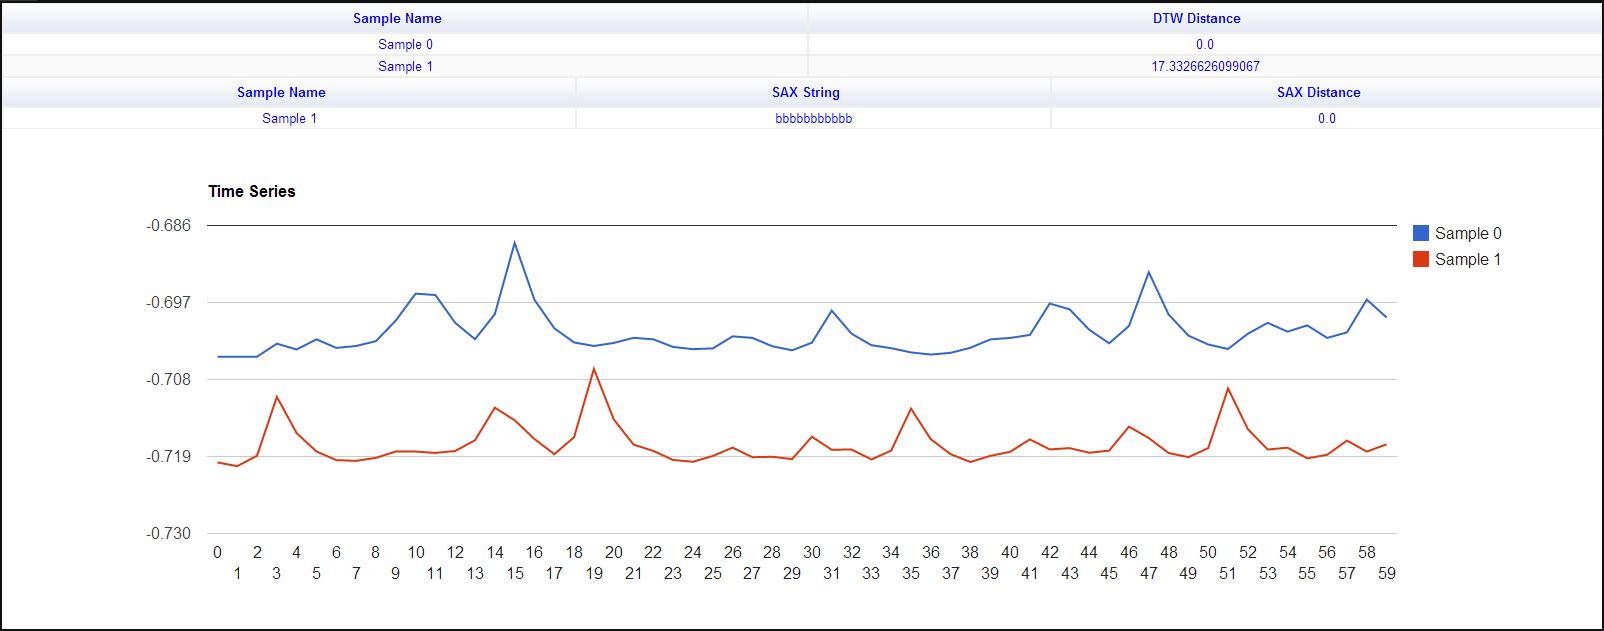
\includegraphics[scale=0.35]{./screenshots/result_sim_sax.png}
  \caption{Similarity detection of two Samples of five years each using SAX and DTW  Algorithm for Shidlaghatta Taluk.}
\end{figure}
\subsubsection{SAX Algorithm }
\paragraph{} In SAX algorithm the time series is converted to a string. The working of this algorithm is shown in the figure 7.2 . The algorithms shows an SAX string representation of the sample and the corresponding similarity between the series.
\begin{figure}[h!]

  \centering
    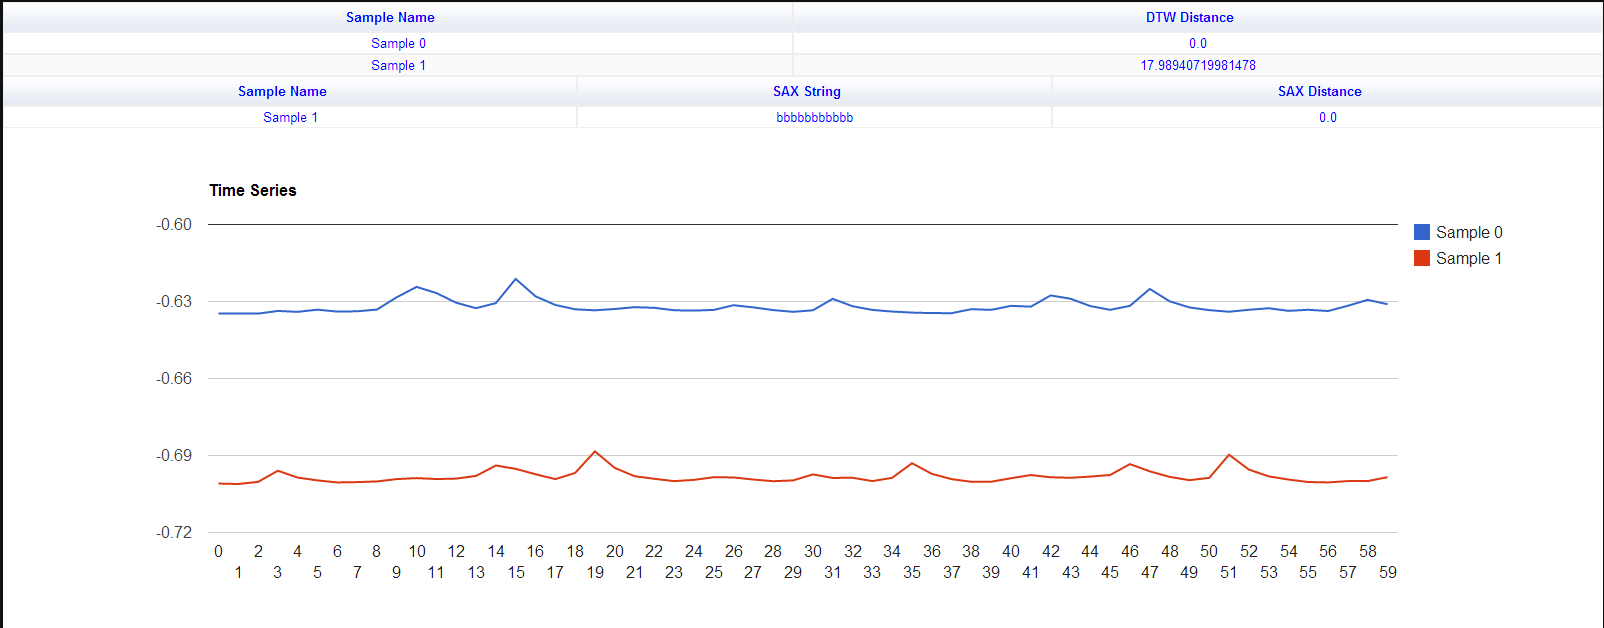
\includegraphics[scale=0.35]{./screenshots/result_sim_sax_2.png}
  \caption{Similarity detection of two Samples of five years each using SAX and DTW  Algorithm for Gowribidanur Taluk .}
\end{figure}
\subsection{Anomaly Detection}
\paragraph{} The anomaly detection algorithms require the user to specify a threshold value. This threshold value  determines the number of anomalous points discovered.
\subsubsection{Cumulative Sum}
\paragraph{} Figure 7.3 shows the anomalous points determined by the CUSUM (Cumulative Sum) Algorithm. These points are shown in red. The threshold value set is -4.0 as shown in the figure.
\begin{figure}[h!]

  \centering
    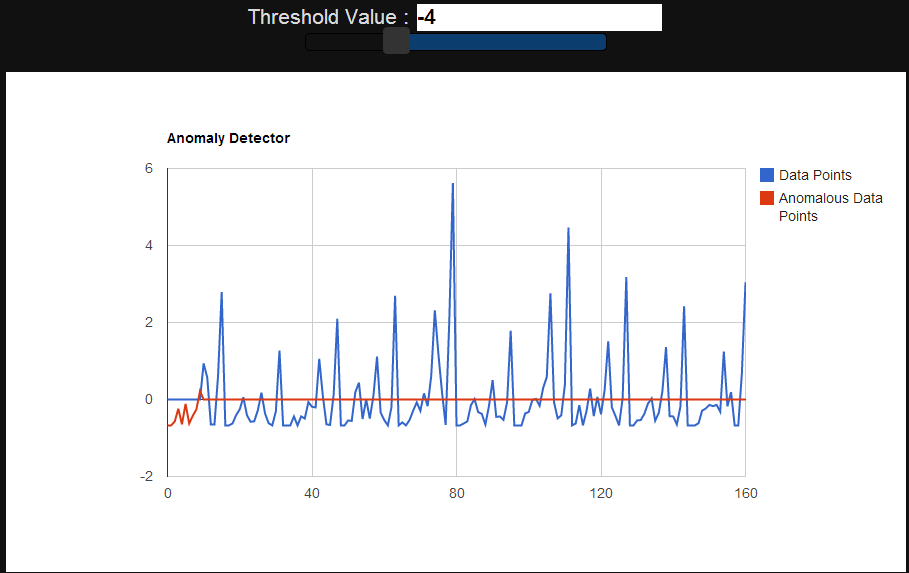
\includegraphics[scale=0.5]{./screenshots/result_ano_cusum_Bag.png}
  \caption{Anomaly detection using the Cumulative Sum Approach for Rainfall data set of Bagepalli Taluk.}
\end{figure}

\subsubsection{Statistical Approach Anomaly}
\paragraph{} In this approach a moving average of the time series is calculated. Then an upper and lower limit is defined as boundary. These limits are basically defined using the standard deviation of the data points. This boundary determines the number of anomalous data points discovered. The figures 7.4 and 7.5 show the mean, upper limit and lower limit in the top graph and the anomalous data points discovered in the bottom graph for the rainfall data sets of Shidlaghatta and Gowribidanur taluks.
\begin{figure}[h!]

  \centering
    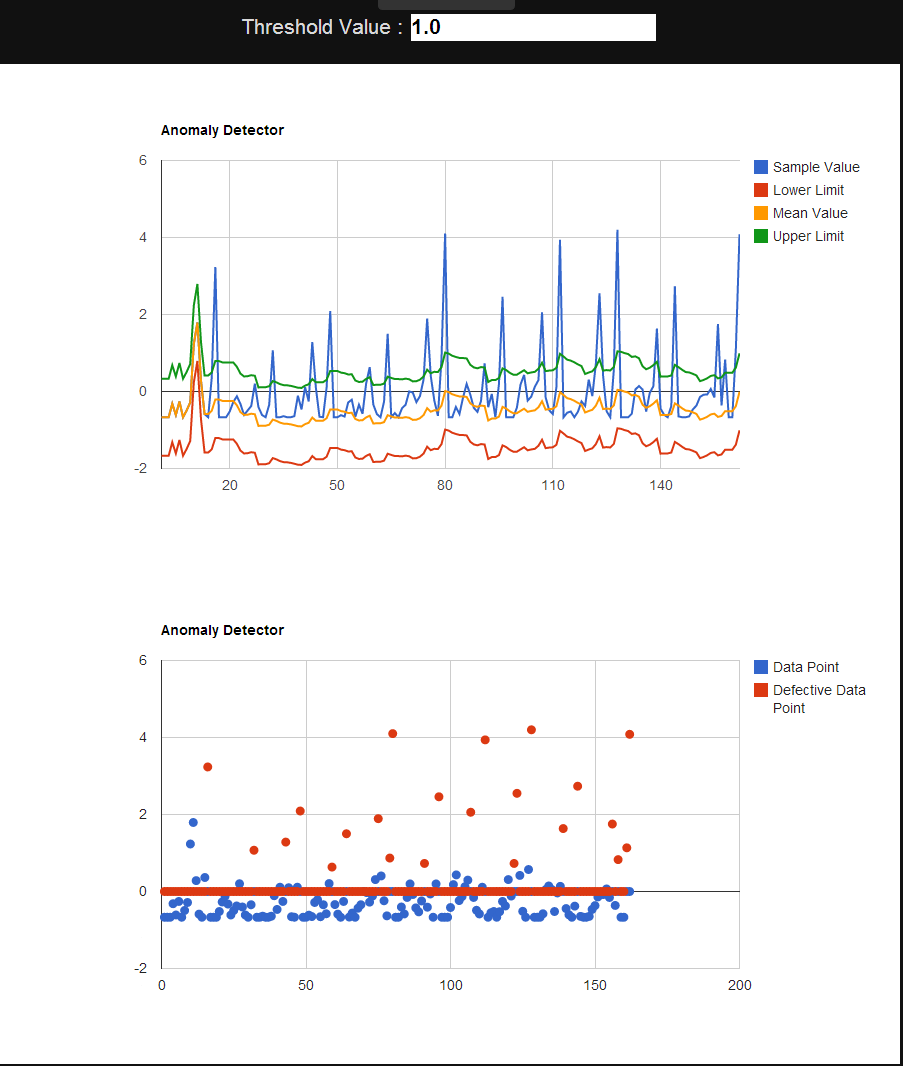
\includegraphics[scale=0.5]{./screenshots/result_ano_stat_Gow.png}
  \caption{Anomaly detection using the Statistical Approach for rainfall data set of Gowribidanuru taluk.}
\end{figure}

\begin{figure}[h!]

  \centering
    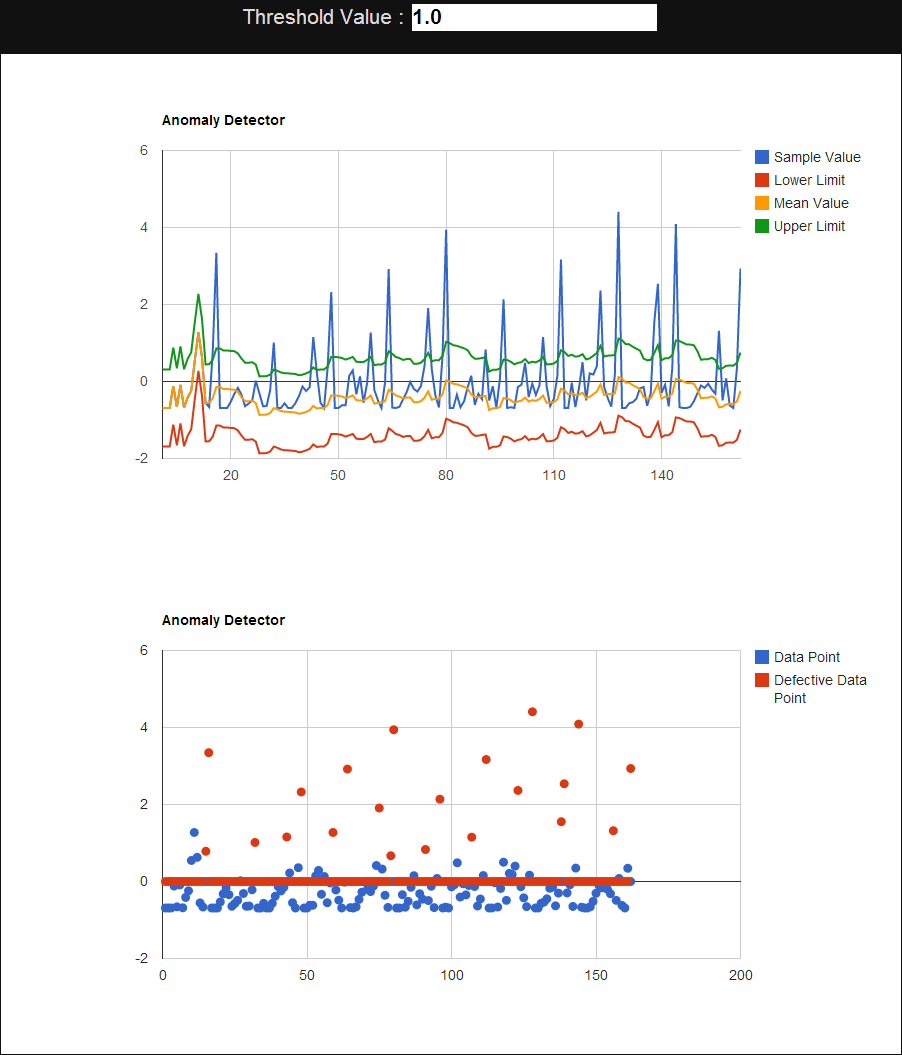
\includegraphics[scale=0.5]{./screenshots/result_ano_stat_Sid.png}
  \caption{Anomaly detection using the Statistical Approach for rainfall data set of Shidlaghatta taluk.}
\end{figure}

\subsection{Prediction and Forecasting}
\subsubsection{NARX Neural Network Approach}
\paragraph{} NARX is Non-Linear Auto Regressive model with Extraneous Inputs. This is basically a neural network which predicts one time series which depends on another time series. A feed forward network with backpropogation algorithm is implemented. 


The results obtained by the neural network are shown in Figures 7.6 and 7.7. The accuracy obtained is around 60\% and it is for the rainfall data sets of Gowribidanuru and Shidlaghatta taluks estimated over  1 year and 2 years span respectively.

Various neural network parameters are :
\begin{itemize}
\item \textbf{Activation Function} : Sigmoidal activation function.
\item \textbf{Hidden Layer Size} : 20 neurons. If more number of neurons are used, he accuracy of the results increase but the computation is expensive.
\item \textbf{Learning Rate } : 0.01 - 0.03. 
\end{itemize}

\begin{figure}[h!]

  \centering
    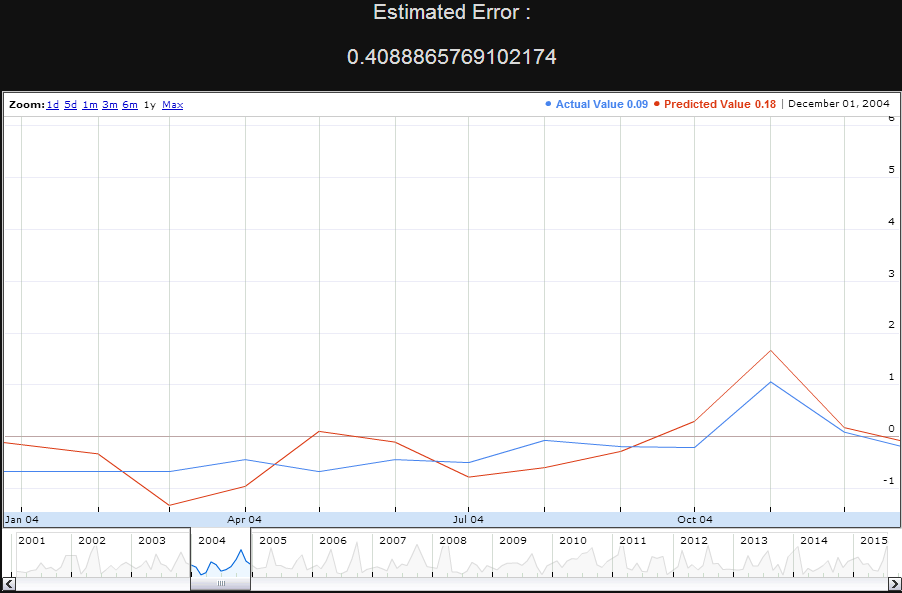
\includegraphics[scale=0.35]{./screenshots/result_fort_NN_Bag.png}
  \caption{Forecasting/Estimation using NARX Neural Network Approach for Rainfall data set of Bagepalli taluk.}
\end{figure}


\begin{figure}[h!]

  \centering
    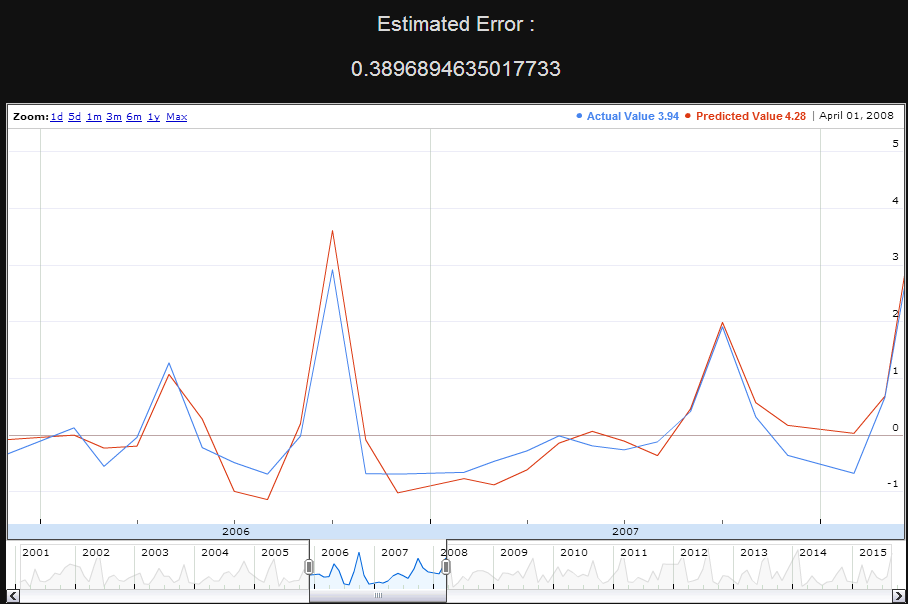
\includegraphics[scale=0.35]{./screenshots/result_fort_NN_Sid.png}
  \caption{Forecasting/Estimation using NARX Neural Network Approach for Rainfall data set of Shidlaghatta taluk.}
\end{figure}
\subsubsection{Moving Exponential Average Method}
\paragraph{} This method computes a moving exponential average and this value computed is the predicted value of the time series. The results obtained are shown in the figures 7.8 and 7.9 for rainfall data sets of Bagepalli and Gowribidanur taluks respectively.




This is not a conventional approach, the value predicted by this algorithm is just an estimation and not an actual prediction. The accuracy of this approach is around 50\%.
\begin{figure}[h!]
  \centering
    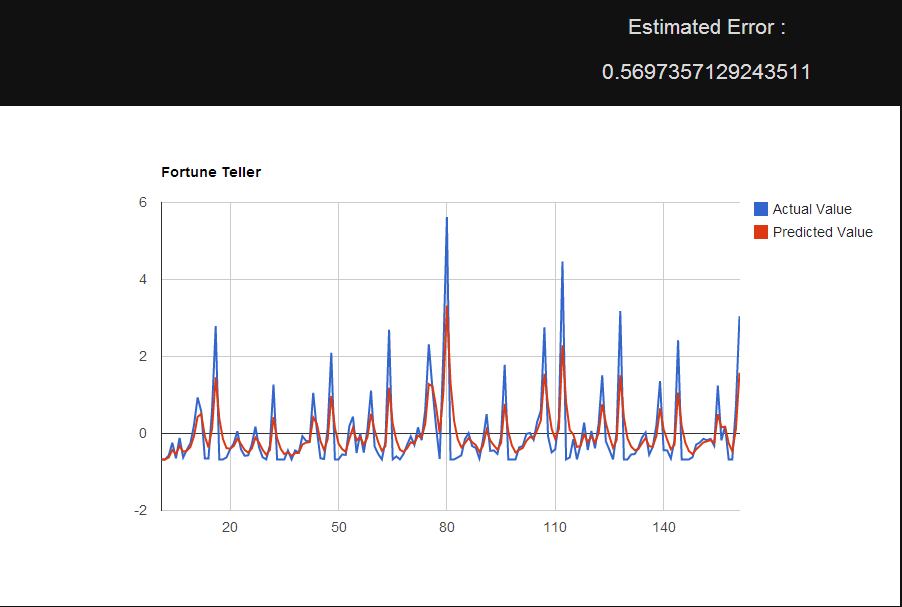
\includegraphics[scale=0.55]{./screenshots/result_fort_MEA_Bag.png}
  \caption{Forecasting/Estimation using Moving Exponential Average Method for rainfall data set of Bagepalli Taluk.}
\end{figure}


\begin{figure}[h!]
  \centering
    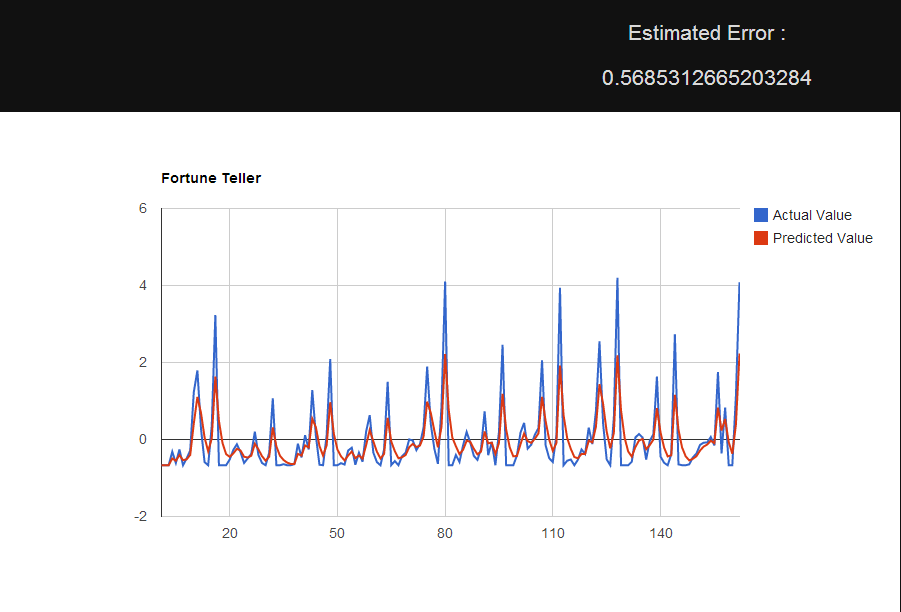
\includegraphics[scale=0.55]{./screenshots/result_fort_MEA_Gow.png}
  \caption{Forecasting/Estimation using Moving Exponential Average Method for rainfall data set of Gowribidanur Taluk.}
\end{figure}
\subsection{Temporal Pattern Detection}
\paragraph{} Temporal Patterns are hidden patterns which occur very rarely. These patterns are basically the indications of periodic trends. In this project, the temporal pattern finder module is implemented using a genetic algorithm. A fitness value is to be set for the algorithm, depending on this value, the patterns are discovered. 

Figure 7.10 shows the patterns discovered in the rain fall data set of Bagepalli taluk.  The patterns are highlighted with red dots in the graphs shown in figure in 7.10.
\begin{figure}[h!]

  \centering
    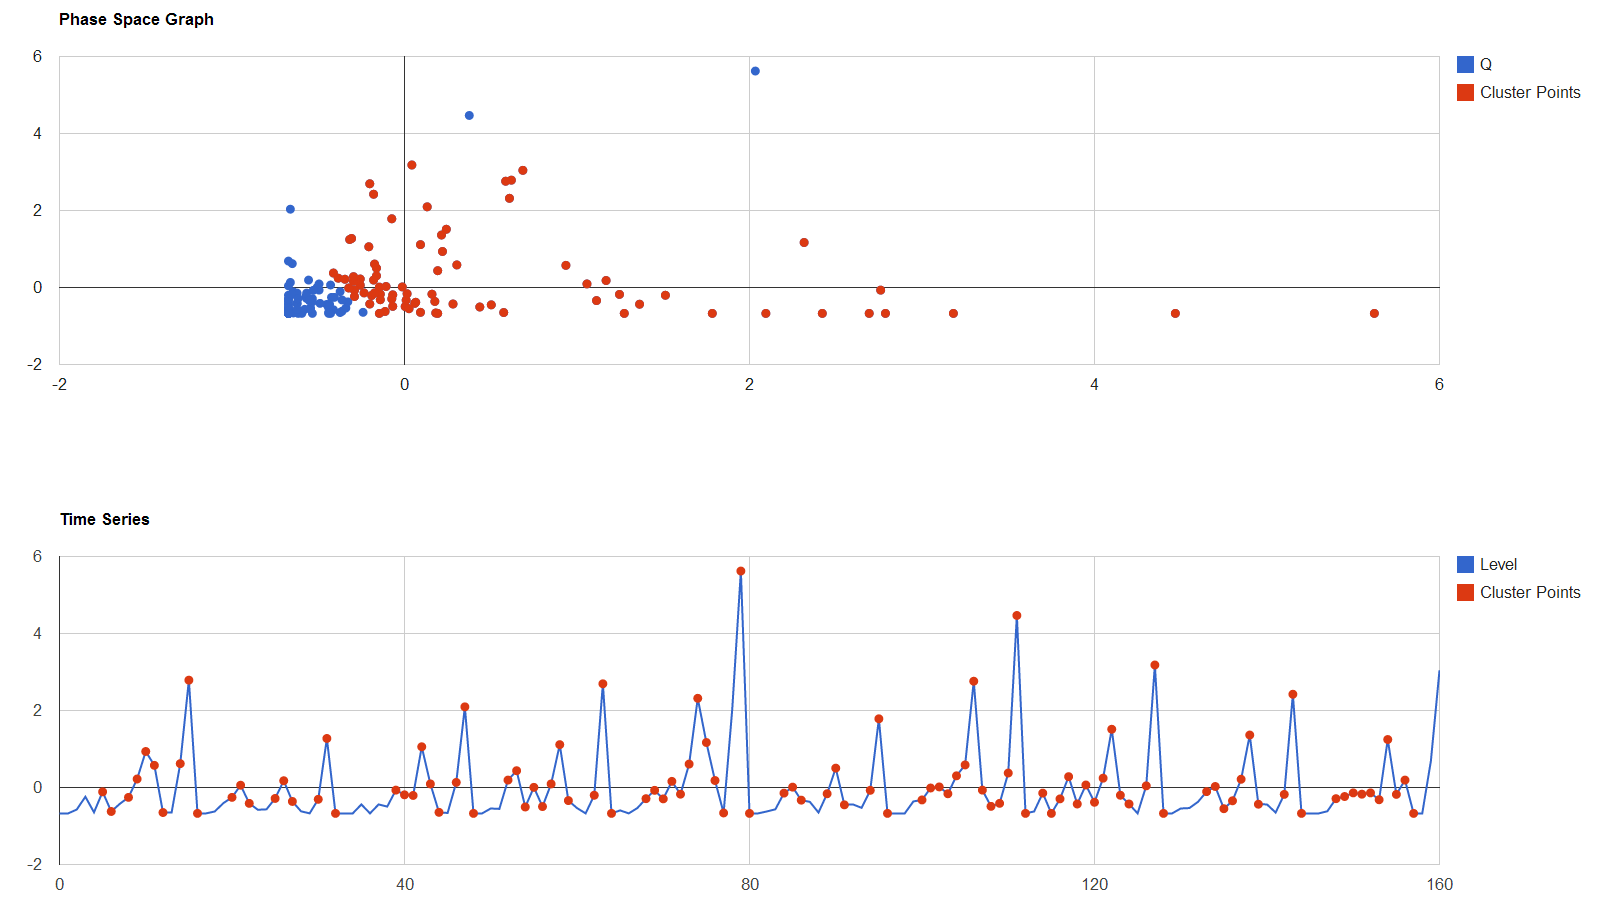
\includegraphics[scale=0.35]{./screenshots/result_tmp_pattern_Bag.png}
  \caption{Temporal Patterns detected in the Rainfall/Water Data set of Bagepalli taluk.}
\end{figure}
\section{Inference from the Results}
\begin{enumerate}

\item \textbf{Forecasting and Prediction}
\begin{itemize}
\item  NARX Neural Network : The accuracy of this algorithms considering various evaluation metrics specified in the previous section is around 60\%. This accuracy can be different for different data sets and depending on the specified parameters like learning rate, hidden layer size, the activation function used.
\item \textbf{ Moving Exponential Method : } This algorithm does not require any special paramters to be specified. The efficiency of this algorithm is around 40\% for water data set.
\item \textbf{Simple Moving Average and Geometrical Moving Average : } These methods are naive and are only estimation techniques and have few low accuracies.
\end{itemize}

\item \textbf{Anomaly Detection }

\begin{itemize}
\item  Statistical Approach 
\item  CUSUM Approach 
\end{itemize}
These anomaly detection algorithms work in specific ways and help in determining the anomalous data points. Depending on application, appropriate algorithm is to be used.
\item \textbf{Similarity Detection }
\begin{itemize}
\item  DTW Algorithm : This algorithms helps in comparing two or more time series considering their euclidian distances and exhaustive comparing. This algorithm is computationally expensive but consumes less memory.
\item  SAX Algorithm : This algorithm converts the time series to a string and hence consumes more memory than the DTW algorithm. Computationally this algorithm is less expensive.
\end{itemize}

\item \textbf{Temporal Pattern Finder}
This module helped in determining interesting/temporal patterns in the time series data. The patterns were highlighted in the graphs. It is upto the user to interpret the patterns/ results shown in the graph.

\end{enumerate}


\pagestyle{fancy}
\lhead{\scriptsize{Conclusion}}
\chead{}
\rhead{\scriptsize{Time Series Data Mining Tool}}
\lfoot{\scriptsize{Dept. of CSE, RVCE, Bangalore.}}
\rfoot{\small{\thepage}}
\cfoot{\scriptsize{Jan 2013 - Jun 2013}}
\renewcommand{\headrulewidth}{0.4pt}
\renewcommand{\footrulewidth}{0.4pt}
\chapter{CONCLUSION}
\section{Summary}
\paragraph{}This project successfully implements the Time Series Data Mining Tool for analyzing the time series and test its performance. This tool mainly contains four modules, they are - \textbf{Similarity Detection, Forecasting and Prediction, Anomaly Detection and Temporal Pattern Finder}, which were successfully implemented and tested. The results obtained were presented in the previous chapter.
\noindent
The description of the modules are below :
\begin{itemize}
\item \textbf{Similarity Detection} : This module helps in finding similarity patterns (that occur at regular intervals in case of periodic time series), comparing different time series data. SAX and DTW are the main algorithms implemented/used in this module.
\item \textbf{Forecasting and Prediction} : This module contain algorithms/models which can be trained from the past time series data and can be used to predict the future values of a time series. 
\item \textbf{Anomaly Detection} : This module contains algorithms that help in indicating anomalous patterns in the time series data analyzed. Anomalies are patterns in time series which deviate from the normal behavior and can indicate fraud/danger depending on the application. For example in an industry which produces the blades, the thickness of the blade can be monitored by a machine as a time series and any deviation from the normal error rate can signal an error in the manufacturing process.
\item \textbf{Temporal Pattern Finder } : This module helps in finding hidden temporal patterns in a time series. This module can be further extended to implement clustering techniques.
\end{itemize}


Initially this project mainly focused on analyzing the sea and water level time series. Later this application was extended to any uni-variate time series data. Users can upload the time series data to be analyzed and get the results instantly. Major data sets used were :
\begin{itemize}
\item Sea Level Dataset : Indicating the sea level at various times of a day.
\item Water Level : Ground Water level data, indicating the ground water level during various months of an year for upto 5 years.
\item Finance Dataset : Consisting of stock index values of  Nifty and Vix collected every minuted for a week.(5 days,during market hours).
\item ECG Dataset : The ECG  voltage values of patients collected every 4ms.(for 10 patients).
\end{itemize}


In this project, we also analyzed the efficiencies of different algorithms for the same tasks and also compared the results for different data sets.Clearly more work needs to be done.


\section{Limitations}
Some of the shortcomings in our project are :
\begin{enumerate}

\item{} The application hangs when analyzing very large data sets (more than 500 MB).
\item{} The application does not support multi-variate time series.
\item{}Some algorithms efficient for a particular data set and may not be efficient for other data set. So user intervention is required in selecting an algorithm for a data set.
\end{enumerate}

\section{Future enhancements}
Some of the future enhancements are :
\begin{enumerate}
\item{The size of the  time series data analyzed is in terms of Mega Bytes. For larger dataset(In terms of GBs) or big data, distributed computing technologies like Hadoop can be used.}
\item{}The application can be extended to analyze multi variate time series data.
\item{The application could be made more responsive by using Threads and Parallel or Cloud Computing}
\item{One more extension could be analyzing twitter post data with respect to time and predicting the trends. This requires NLP, but is an example of time series.}
\item{Efficient algorithms using Support Vector Models (SVMs) for forecasting, Hidden Markov Model for anomaly detection can be implemented.}
\item{This application uses static time series data, enhancements can be made to use real time data.(In finance applications)}

%\item{This application can be converted into an mobile application (android, iPhone, iPad) where the users can analyze the time series data on the go and share the results on facebook}

\end{enumerate}



%For Bib refer to refs.bib to add/remove bib items
\addcontentsline{toc}{section}{REFERENCES}
\begin{thebibliography}{refs}
\bibitem{t}
 Robert H. Shumway, David S. Stoffer
 \textit{Time Series Analysis and Its Applications: With R Examples, Springer, 2011}

\bibitem{te}Antunes C.M., Oliveira A.L., \textit{``Temporal Data Mining: An Overview"}, Workshop on Temporal Data
Mining ACM SIGKDD 2010, San Francisco, California (USA), August 2010.

\bibitem{t}Agrawal R., Lin K.-I., Sawhney H. S., Shim K., \textit{``Fast Similarity Search in the Presence of Noise,
Scaling, and Translation in Time-Series Databases"}, Proc. VLDB 1995, pp. 490-501, Zurich
(Switzerland), September 2008.

\bibitem{t}
Damle; Chaitanya, Yalcin; Ali - 
\textit{Flood prediction using Time Series Data Mining}
Journal of Hydrology, Volume 333, Issues 2–4, 15 February 2007, Pages 305 – 316.

\bibitem{t} Berndt D. J., Clifford J., \textit{“Using Dynamic Time Warping to Find Patterns in Time Series”}, KDD
Workshop 2004, pp.359-370, Seattle, WA (USA), July 2004.

\bibitem{t} Faloutsos C., \textit{“Mining Time Series Data”}, Tutorial ICML 2003, Washington DC (USA), August 2003.
\bibitem{t}
Keogh, E., Lonardi, S., Chiu, W. \textit{Finding Surprising Patterns in a Time Series
Database In Linear Time and Space}. In the 8th ACM SIGKDD International
Conference on Knowledge Discovery and Data Mining; 2002 Jul 23 – 26;
Edmonton, Alberta, Canada, pp 550-556.
\bibitem{t}Ge, X., Smyth, P. -\textit{Deformable Markov Model Templates for Time-Series Pattern
Matching}. Proceedings of 6th ACM SIGKDD International Conference
on Knowledge Discovery and Data Mining; 2000 Aug 20-23; Boston , MA,pp. 81-90.

\bibitem{t}
Povinelli; Richard J., \textit {Time Series Data Mining: Identifying Temporal patterns for characterization and prediction of time series events}, Milwaukee, Wisconsin
December, 1999.
\bibitem{t}Das G., Lin K.I., Mannila H., Ranganathan G., Smyth P., \textit{“Rule Discovery from Time series”}, Proc.
ACM SIGKDD 1998, pp. 16-22, New York, New York (USA), August 1998.

\bibitem{t}
Ripley, B.D. Pattern recognition and neural networks. Cambridge University
Press, Cambridge, UK, 1996.

\bibitem{t}
Hamilton, James 
\textit{ Time Series Analysis published by Princeton University Press, 1994}

\bibitem{t}
Ann Ratanamahatana; Chotirat, Lin; Jessica, Gunopulos; Dimitrios, Keogh;Eamonn
 Riverside, Vlachos;Michail, Das; Gautam -
\textit{Mining Time Series Data}
University of California,IBM T.J. Watson Research Center, University of Texas, Arlington.
\bibitem{t}
Brown, Robert Goodell (1963).
\textit{Smoothing Forecasting and Prediction of Discrete Time Series. }
Englewood Cliffs, NJ: Prentice-Hall.
\bibitem{t}
Kurt Pohlen
\textit{The Review of Economics and Statistics}
Vol. 11, No. 3 (Aug., 1929), pp. 149-151
Published by: The MIT Press

\end{thebibliography}

\newpage
\pagestyle{fancy}
\lhead{\scriptsize{Appendix A: Screen Shots}}
\chead{}
\rhead{\scriptsize{Time Series Data Mining Tool}}
\lfoot{\scriptsize{Dept. of CSE, RVCE, Bangalore.}}
\rfoot{\small{\thepage}}
\cfoot{\scriptsize{Jan 2013 - Jun 2013}}
\renewcommand{\headrulewidth}{0.4pt}
\renewcommand{\footrulewidth}{0.4pt}

%\addcontentsline{toc}{section*}{APPENDICES}
%\section*{Appendices}
%%\section*{Appendix A : Source Code}
%\section*{Appendix A : Screen Shots}
%\begin{figure}[h!]
%
%  \centering
%    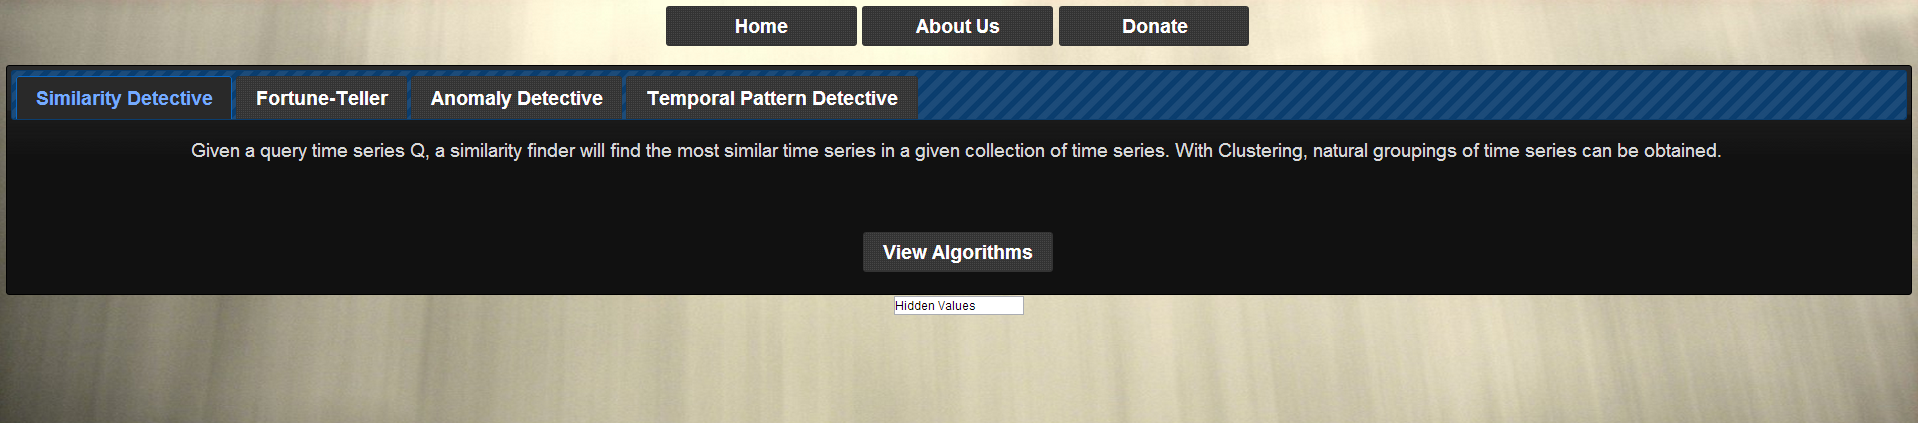
\includegraphics[scale=0.30]{./screenshots/welcome_screen.png}
%  \caption{TSDM Tool Window - Welcome Screen}
%\end{figure}
%
%\begin{figure}[h!]
%  
%  \centering
%    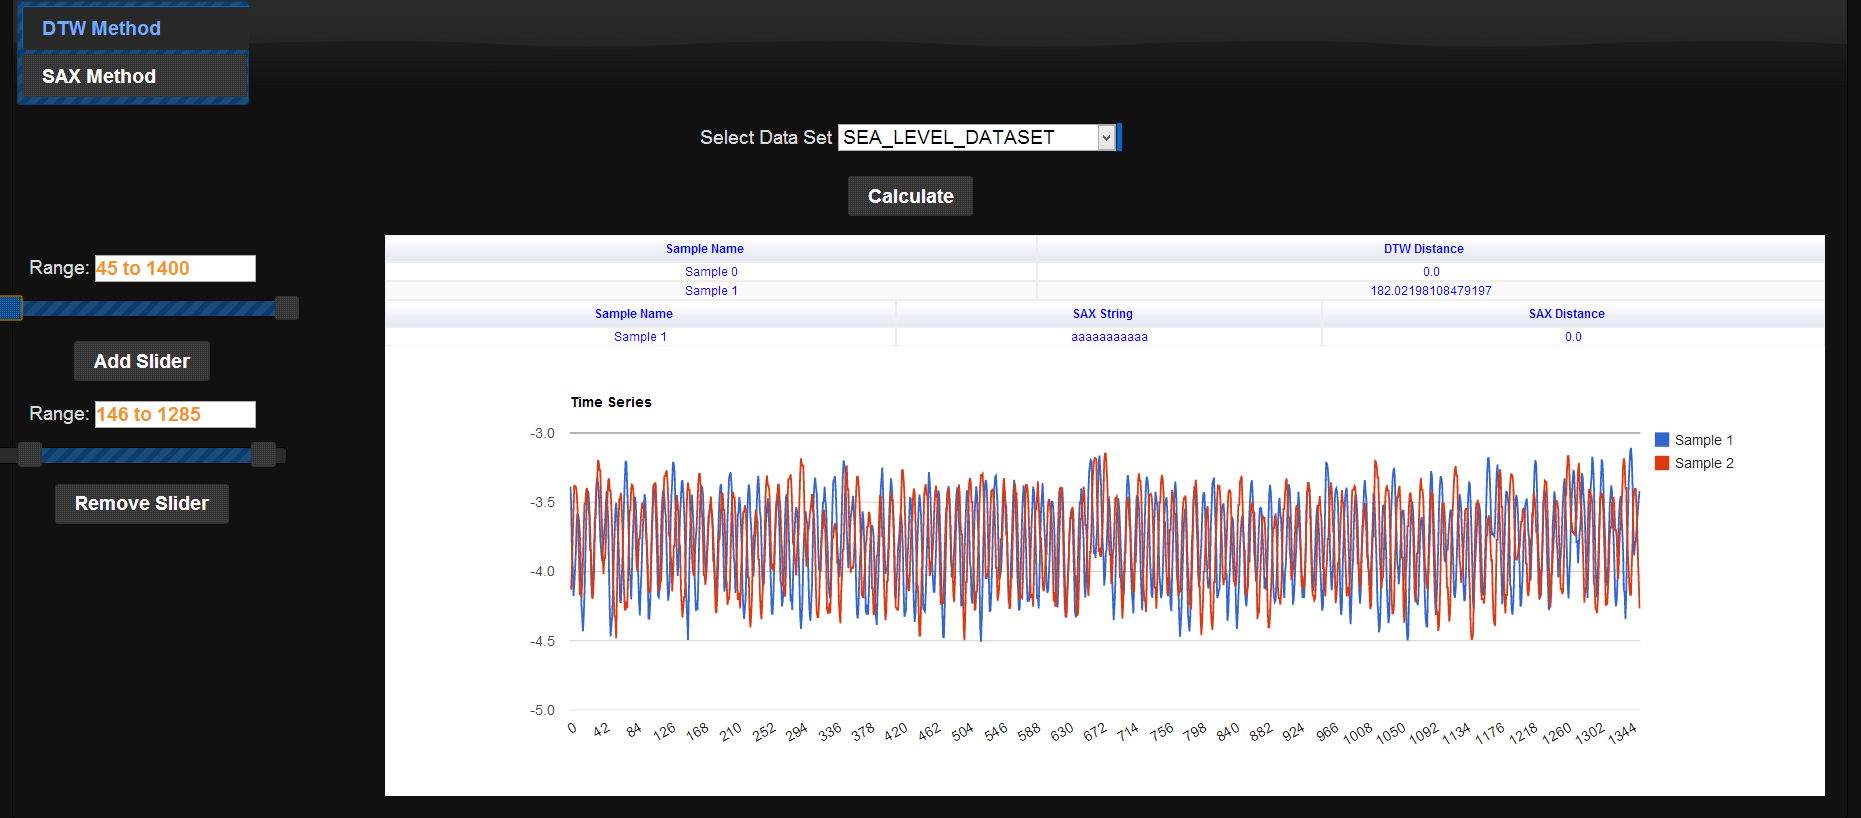
\includegraphics[scale=0.30]{./screenshots/sim_dtw.png}
%\caption{Similarity Detection with DTW Algorithm.}
%\end{figure}
%
%\begin{figure}[h!]
%  
%  \centering
%    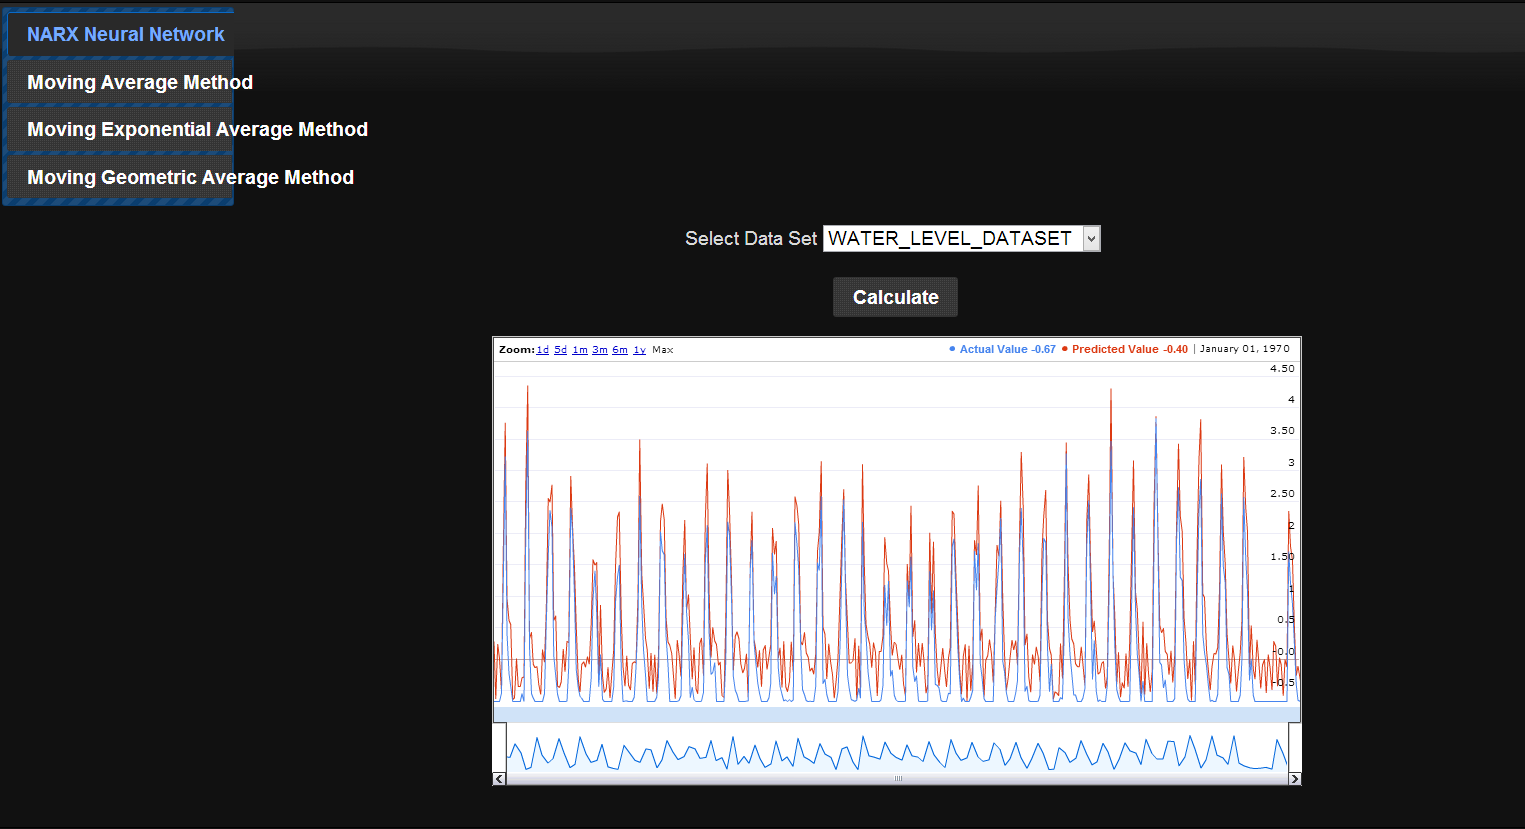
\includegraphics[scale=0.40]{./screenshots/ft_narx.png}
%\caption{Time Series Prediction with NARX NN Model.}
%\end{figure}
%\begin{figure}[h!]
%  
%  \centering
%    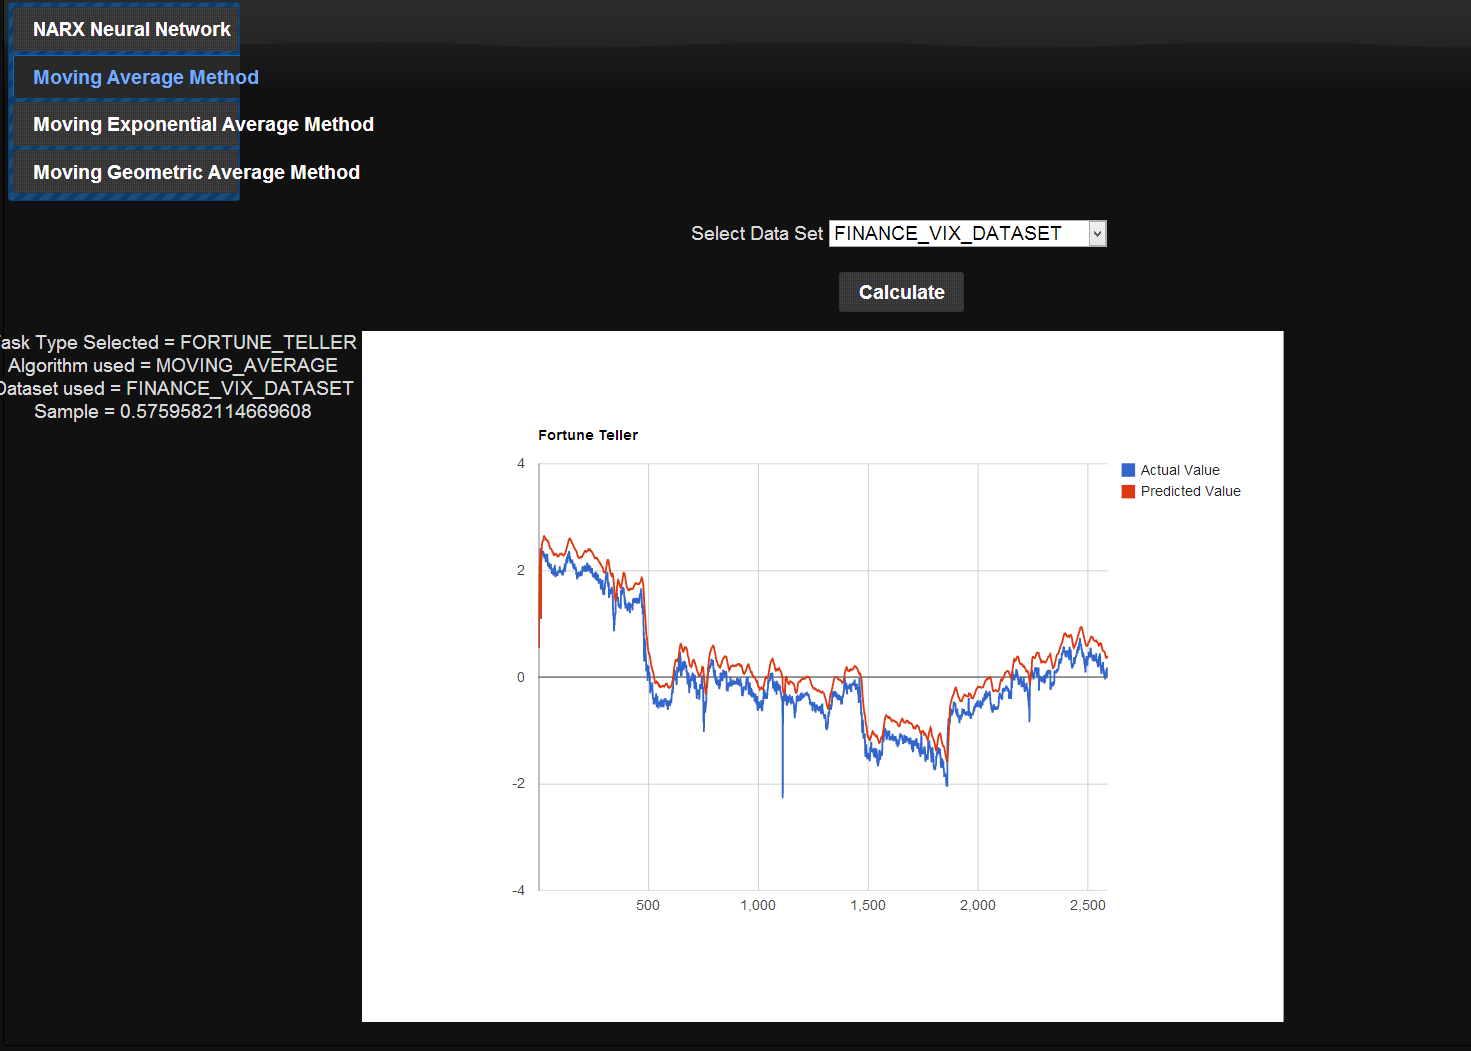
\includegraphics[scale=0.400]{./screenshots/ft_mv_avg.png}
%\caption{Time Series Prediction with Moving Average Method.}
%\end{figure}
%
%\begin{figure}[h!]
%  
%  \centering
%    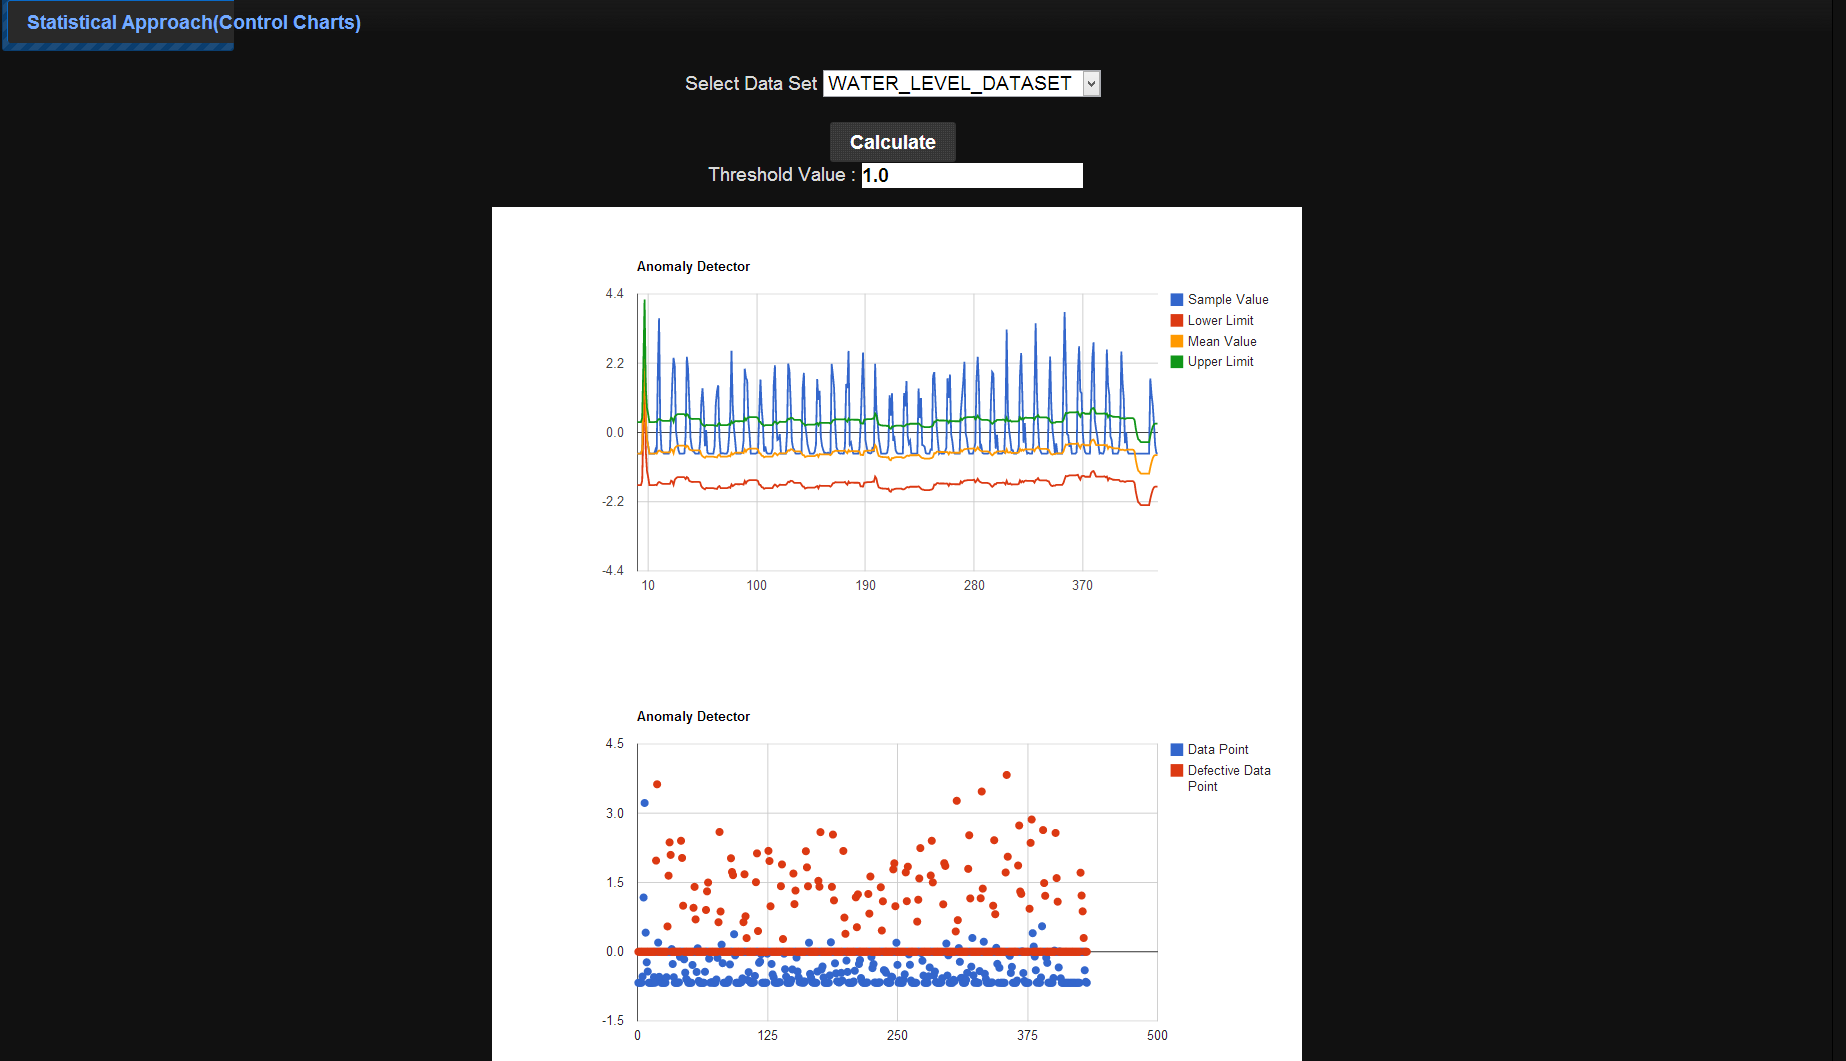
\includegraphics[scale=0.30]{./screenshots/ano_stat_app.png}
%\caption{Anomaly Detection using Statistical Approach.}
%\end{figure}
%
%\begin{figure}[h!]
%  
%  \centering
%    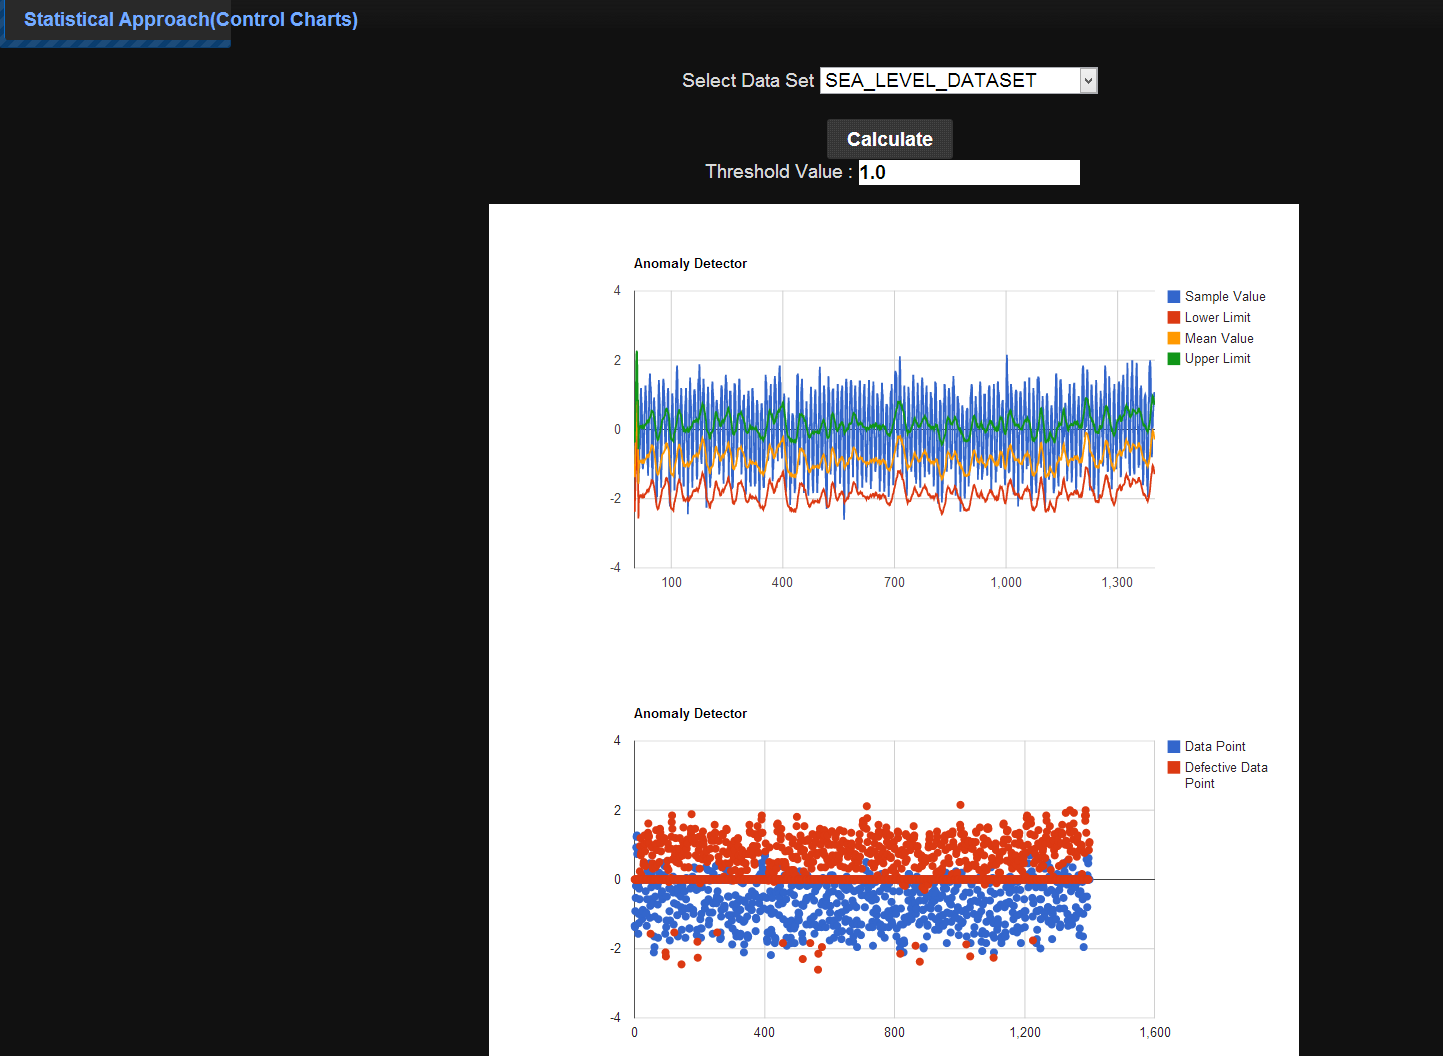
\includegraphics[scale=0.350]{./screenshots/ano_stat_app_2.png}
%\caption{Anomaly Detection using Cusum Algorithm.}
%\end{figure}
%
%\begin{figure}[h!]
%  
%  \centering
%    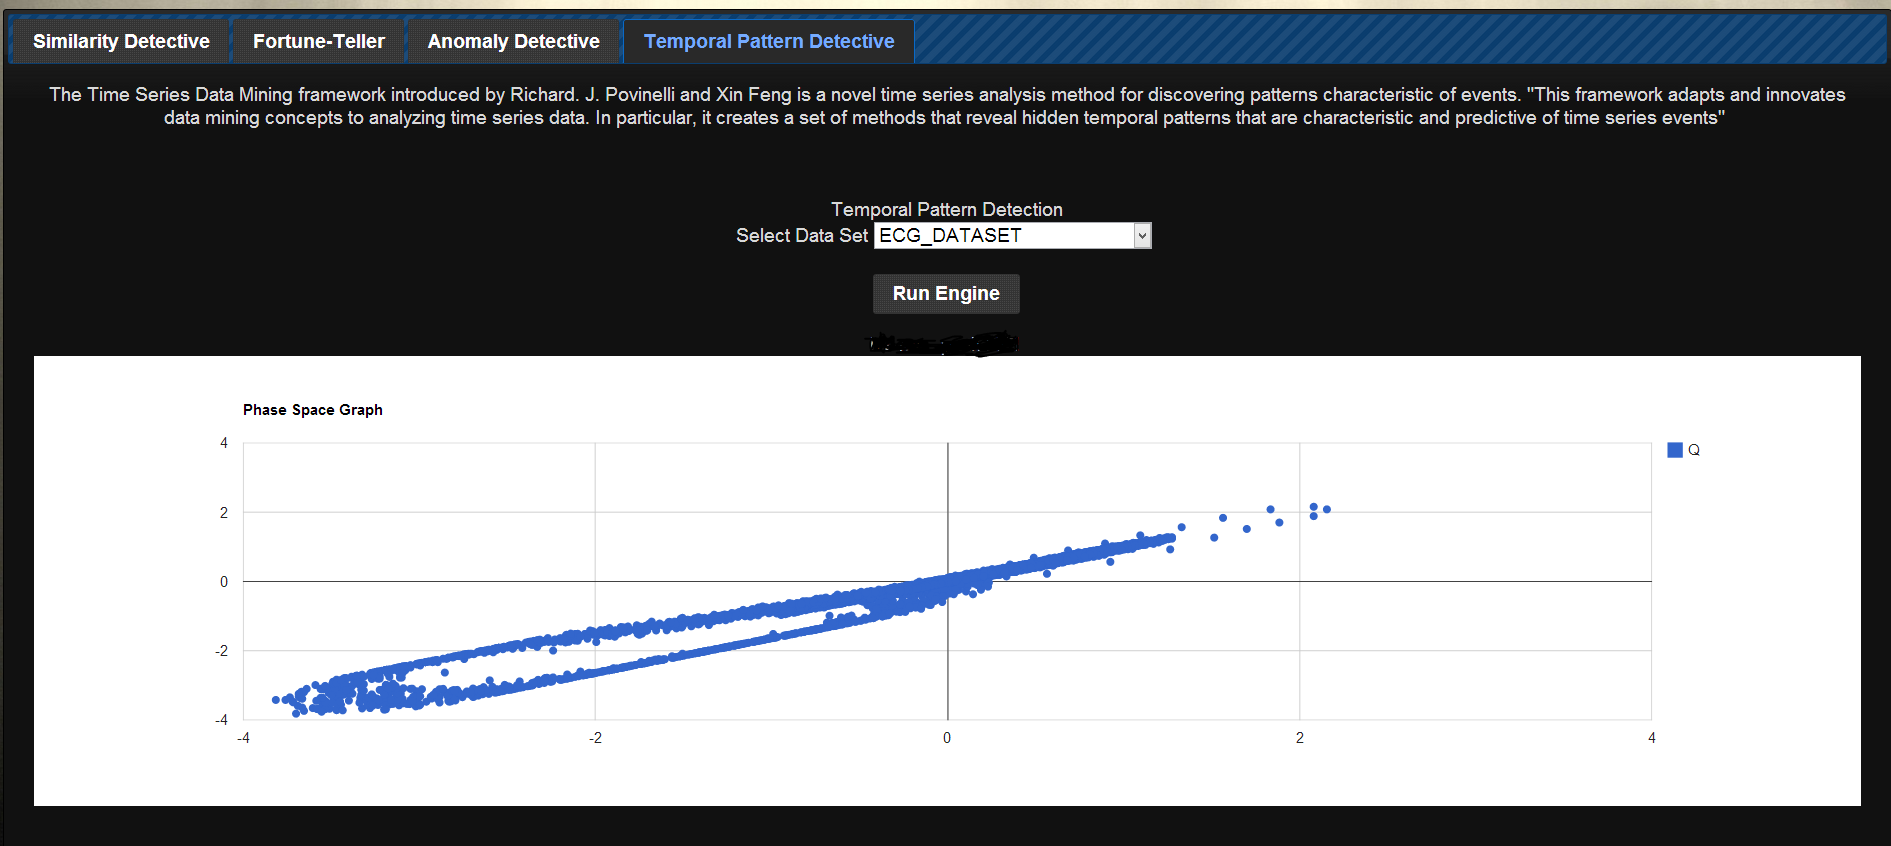
\includegraphics[scale=0.30]{./screenshots/temp_pattern.png}
%\caption{Temporal Pattern Detection using Phase space diagram.}
%\end{figure}
%\begin{figure}[h!]
%  
%  \centering
%    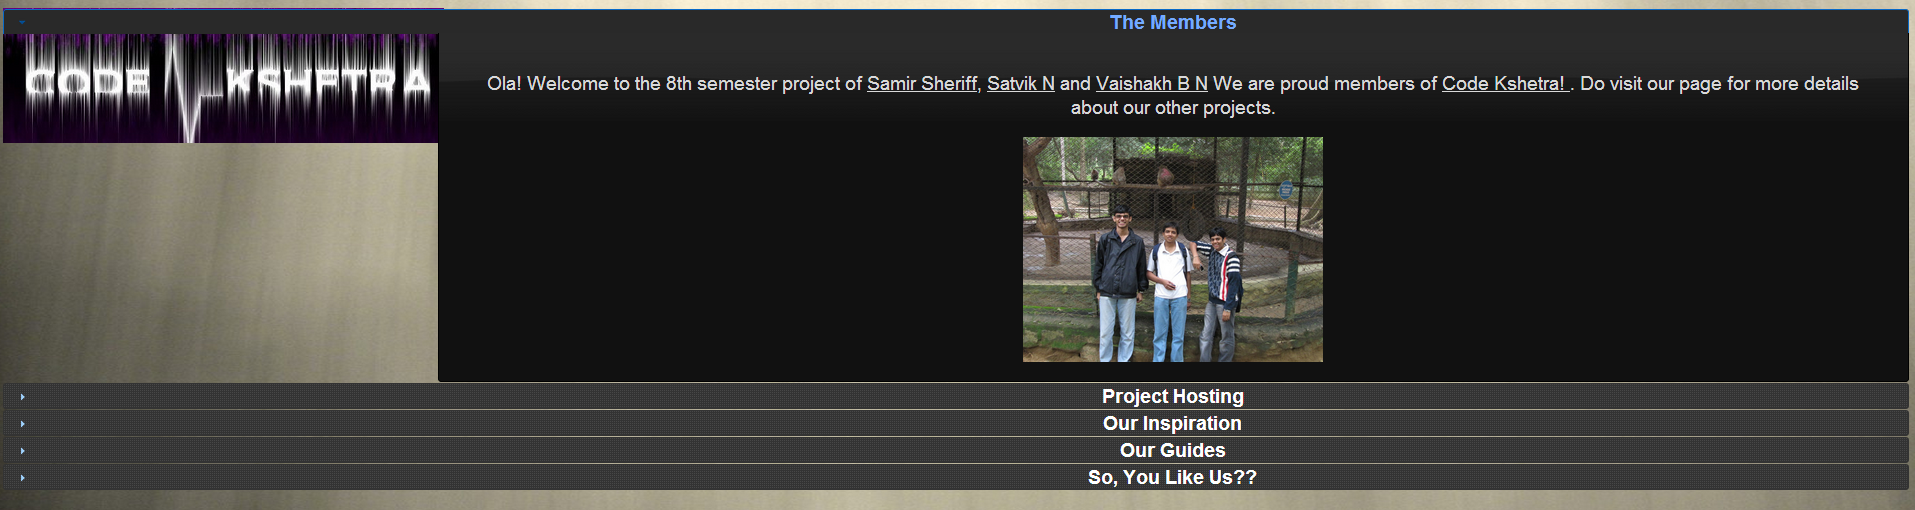
\includegraphics[scale=0.30]{./screenshots/about_us.png}
%\caption{About the Developers who did this project!}
%\end{figure}
%\begin{figure}[h!]
%  
%  \centering
%    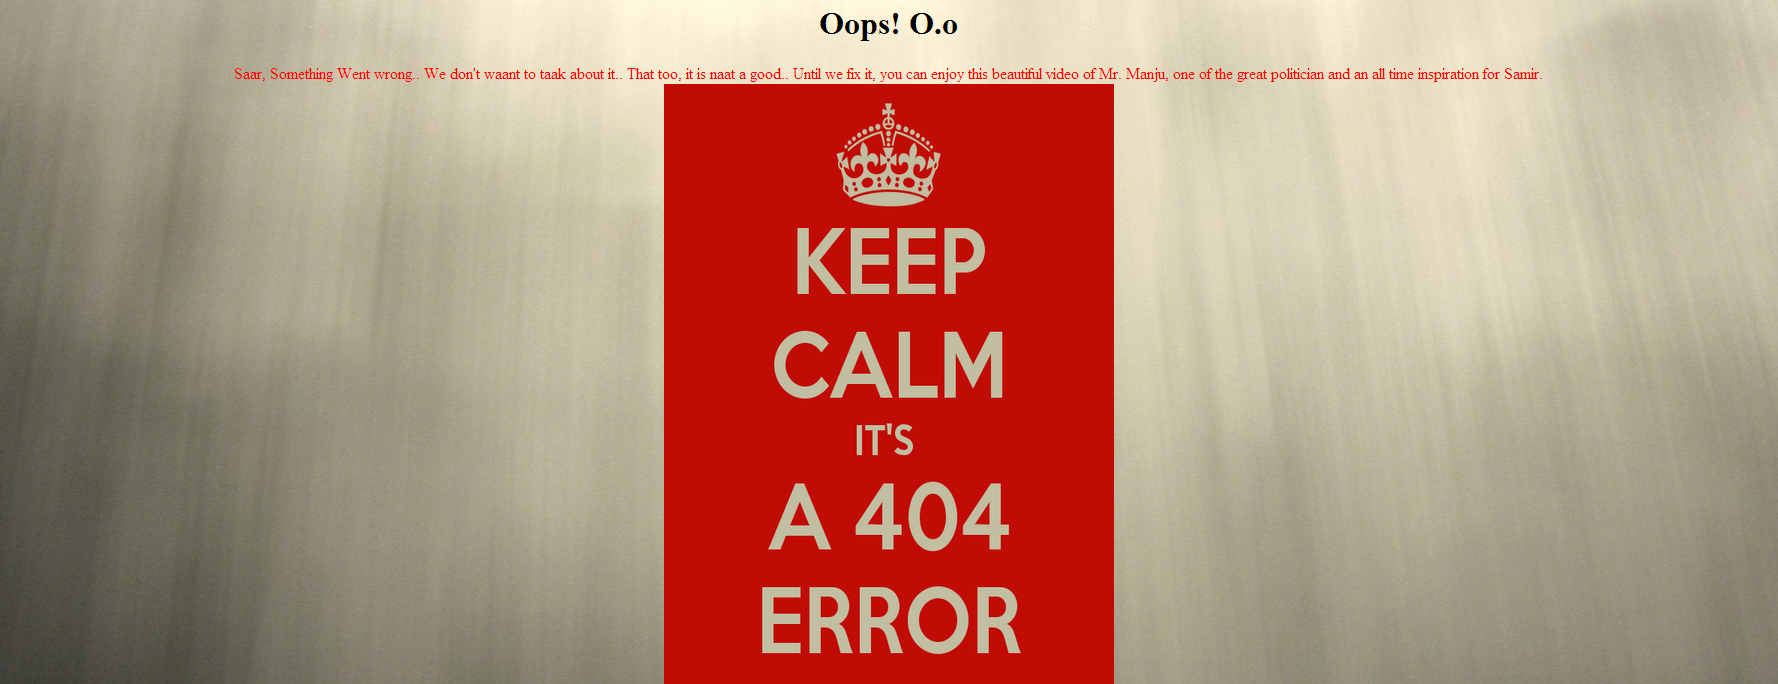
\includegraphics[scale=0.30]{./screenshots/error_page.png}
%\caption{404 File not found error page.}
%\end{figure}
%\lstinputlisting[language=Java, caption=DecisionTreeConstructor.java, breaklines=true]{../../src/org/ck/dt/DecisionTreeConstructor.java}
%\lstinputlisting[language=Java, caption=DecisionTreeClassifier.java, breaklines=true]{../../src/org/ck/dt/DecisionTreeClassifier.java}


%\newpage
%\pagestyle{fancy}
%\lhead{\scriptsize{Appendix B: Paper Publication}}
%\chead{}
%\rhead{\scriptsize{Time Series Data Mining Tool}}
%\lfoot{\scriptsize{Dept. of CSE, RVCE, Bangalore.}}
%\rfoot{\small{\thepage}}
%\cfoot{\scriptsize{Jan 2013 - Jun 2013}}
%\renewcommand{\headrulewidth}{0.4pt}
%\renewcommand{\footrulewidth}{0.4pt}
%
%Add Paper to be published in IEEE.

\end{document}
